\documentclass[11pt]{beamer}
\setbeamertemplate{caption}[numbered]
\usetheme{CambridgeUS}
\usepackage[utf8]{inputenc}
\usepackage{amsmath}
\usepackage{amsfonts}
\usepackage{amssymb}
\bibliography{biblio}
\author{Qilun Lyu}
\title{The Interference of Pandemic to Aviation Performance}
%\setbeamercovered{transparent} 
%\setbeamertemplate{navigation symbols}{} 
%\logo{} 
\date{05/03/2021} 
\institute{Rutgers University} 
\subject{MSDS597} 

\begin{document}
\begin{frame}
\titlepage
\center \small
ql193@rutgers.edu \\
(908)930-8642
\end{frame}

\begin{frame}{Introduction}
\begin{itemize}
\item Delay or cancellation of flights leads to time and profit loss for all the parties engaged: passengers,  airport authorities,  airline companies.
\item On-Time Performance (OTP) or punctuality is regarded by the
majority as the most primary Key Performance Indicators
(KPI) of an airline's rating on the top of others (e.g. quality,
price, etc).  
\item  COVID-19 pandemic is still burning,  bringing less profit
to airports and airlines. The gradually formed new norm
make forecasting necessary since it broke
out. 
\end{itemize}
\end{frame}

\begin{frame}{Introduction}
\begin{itemize}
\item All models are wrong! But we can extract useful information for forecasting,  given a decade of records.

\item The project aims to forecast {\bf Cancellation
Rates(CR)}, {\bf On-Time Rates(OTR)}, and {\bf Average Delay Minutes(ADM)} through leveraging
ARIMA models from time-series approaches.

\item To make better comparison, we regard {\it the pandemic} as our only controlled factor, rid of seasonal effects.  We left the last few months of records to evaluate the model fit.
\end{itemize}
\end{frame}

\begin{frame}{Data Description}
\begin{description}[Other description]
  \item[Source] Bureau of Transportation Statistics of United State (BTS)
  \footnote{\url{https://transtats.bts.gov/Fields.asp?gnoyr_VQ=FGJ}}
  \item[Scope] From Jan 2011 to Dec 2020,  120 files in total, one month each; Covering US domestic flights
  \item[Snippet] Shown below
\end{description}
\begin{table}[h!] 
\tiny
\centering
 \begin{tabular}{|c|c|c|c|c|c|c|c|c|}
  \hline 
 Date & Airline & Num & Origin & Dest & DepDelayMin & ArrDelayMin & Cancelled & Diverted\\ 
  \hline 
  2020/05/03 & AA & 1 & JFK & LAX & 1 & 16 & 0 & 0 \\ 
  2020/05/05 & DL & 725 & EWR & ATL & 40 & 3 & 0 & 0 \\ 
  2020/05/07 & AS & 15 & BOS & SEA & 0 & 0 & 1 & 0 \\ 
   \hline
 \end{tabular} 
 \end{table}
 \small
 Every flight is either on-time, delay, canceled, or diverted.  From observations, the portion of diverted flights can be ignored. Thus,  cancellation and execution (normal or delayed) are strongly negatively correlated.
\end{frame}

\begin{frame}{Logic of Processing}
\begin{enumerate}
\large
\item Data Wrangling and Exploration \\
{\small Removing NAs,  Unifying types and Converting to data frames}
\item Model Fitting and Tuning \\
{\small Find a proper set of coefficients for ARIMA(p,d,q)}
\item Residual Analysis \\
{\small Draw residual plots and normality checks}
\item Forecasting and Verification \\
{\small Create prediction intervals and compare to the true data}
\end{enumerate}
\end{frame}
 
\begin{frame}{Data Wrangling}
Though data is in csv format, using {\it read.csv} might mess up the structure, especially when quotation mark appears.  Instead, we adopted \\
\begin{itemize}
\small
\item fread(file=file, sep = ",", stringsAsFactors = FALSE, header = TRUE) 
\end{itemize}
The header of the files before 2020 are of camel-back style, but fully capitalized after that with naming discrepancy.  
\begin{figure}
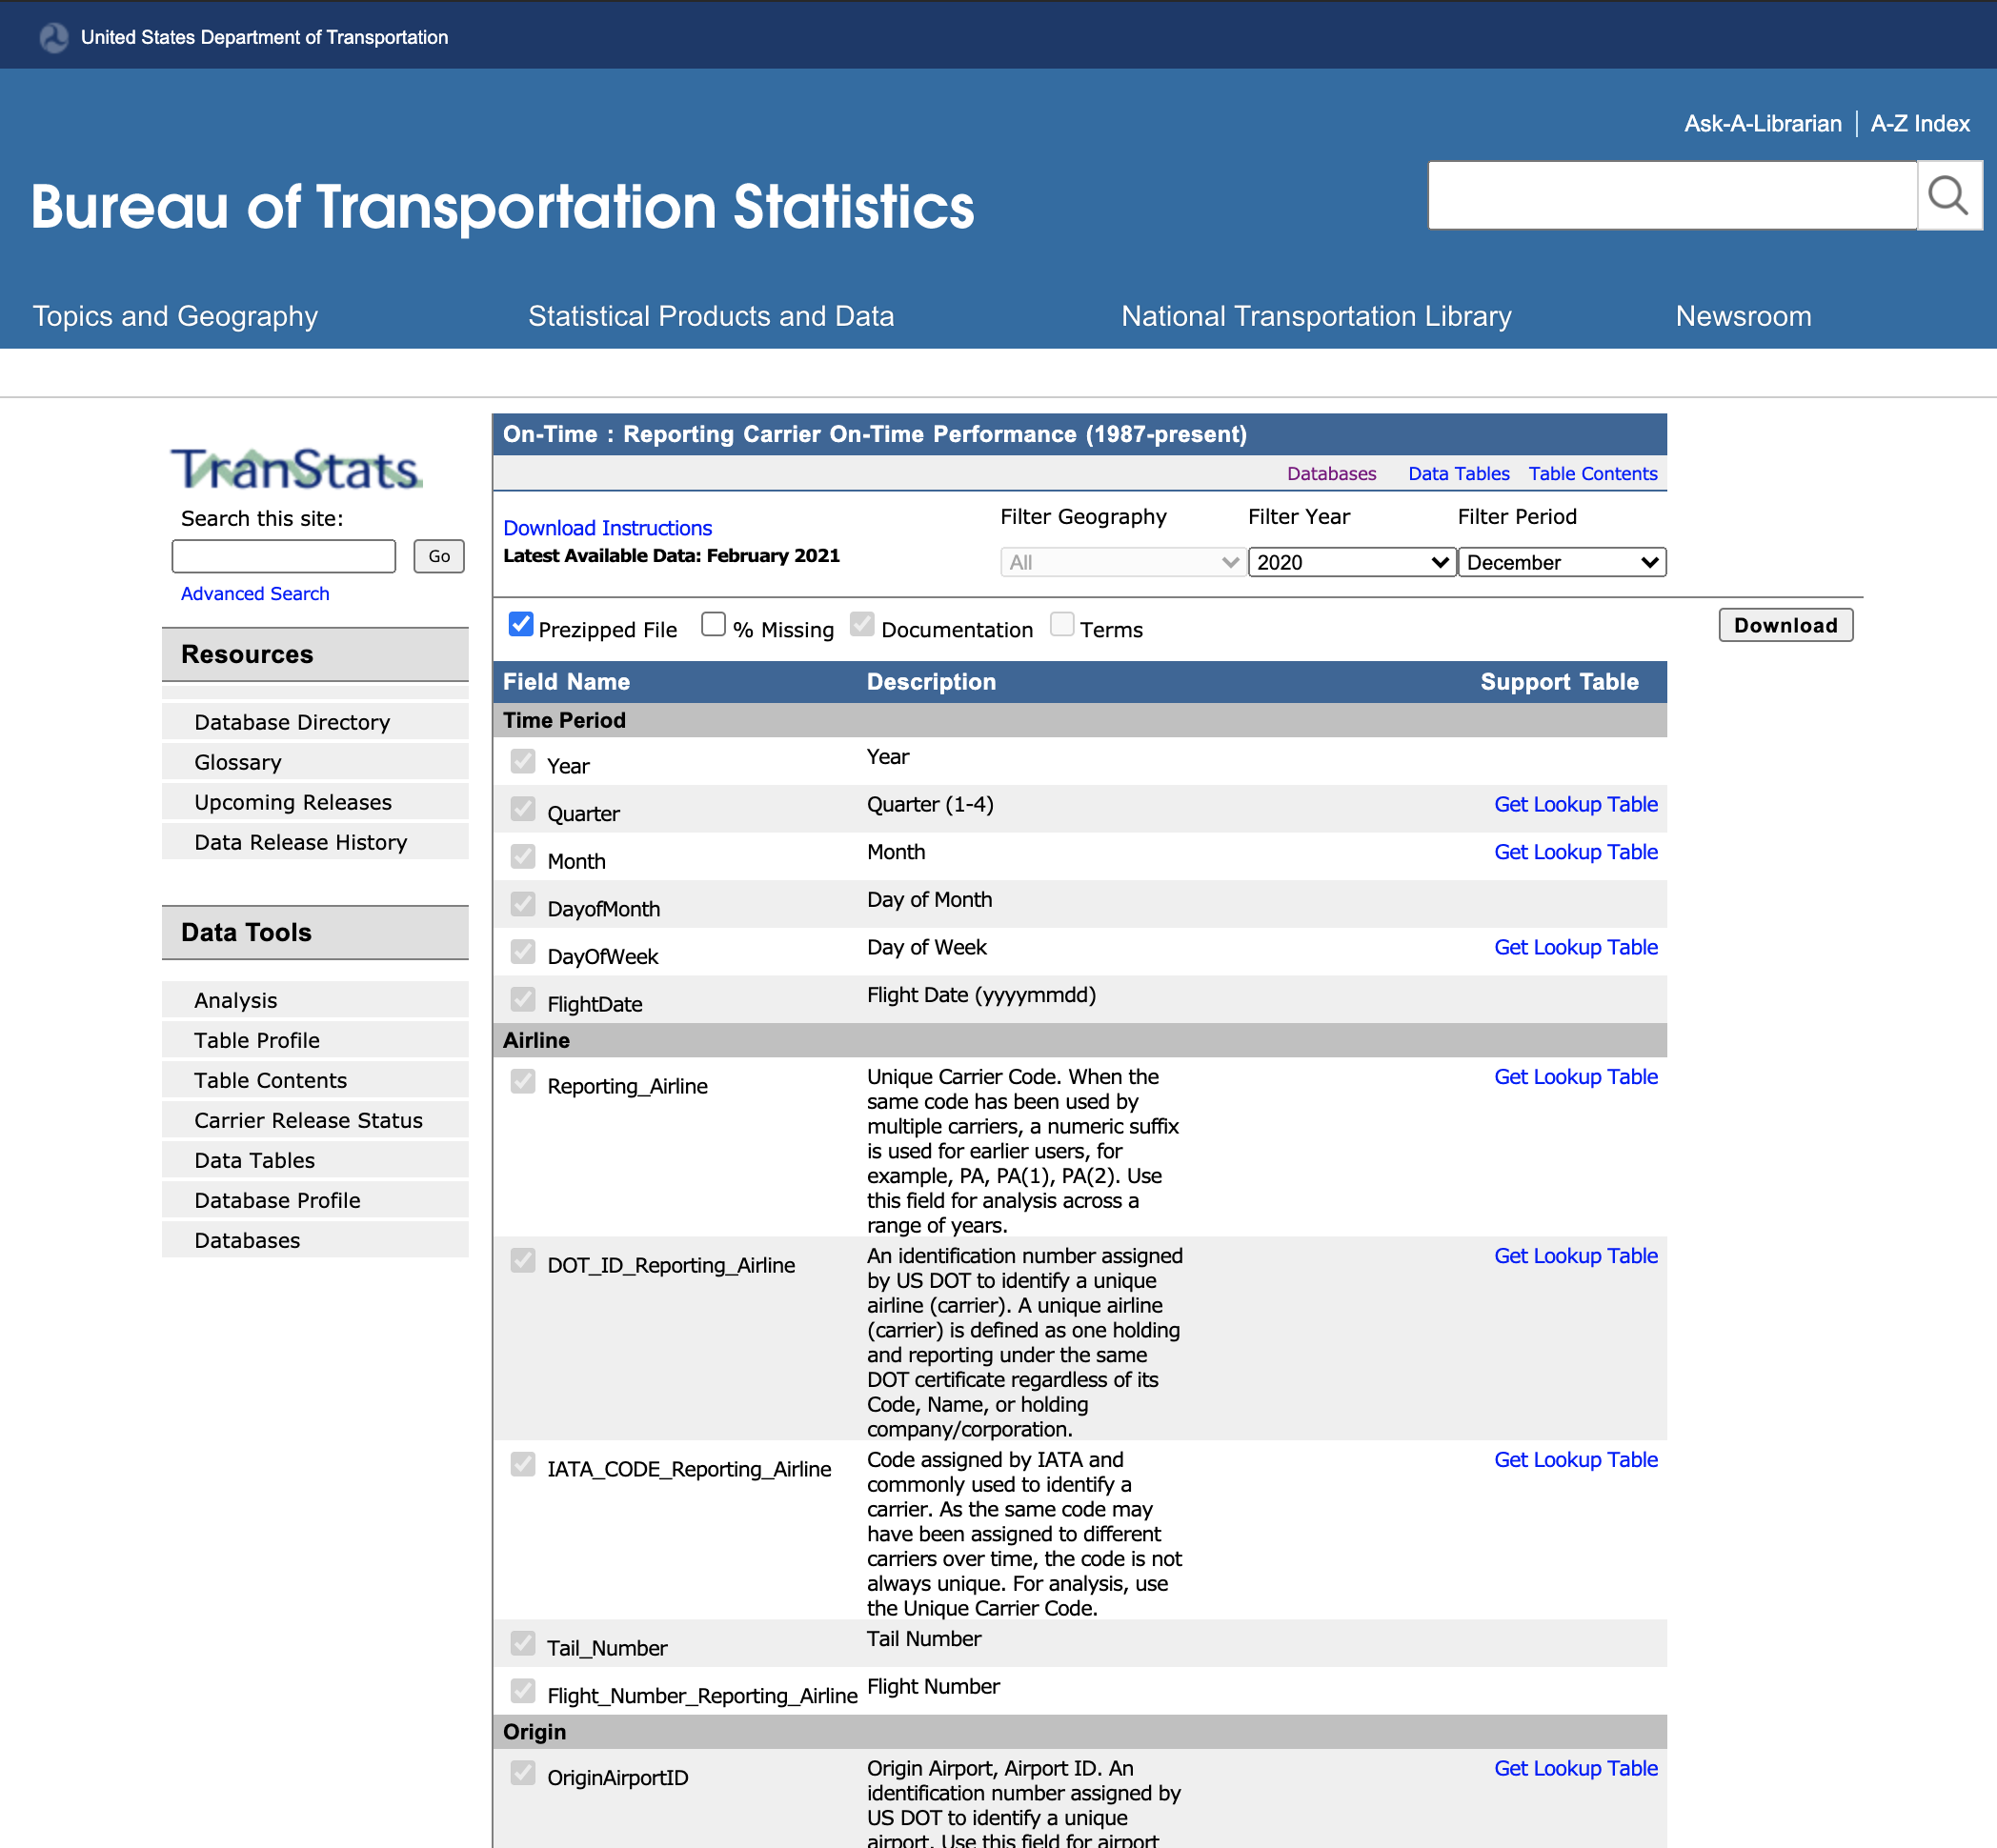
\includegraphics[scale=0.13]{BTSwebsite.png} 
\small
\caption{Data frame}
\end{figure}
\end{frame}

\begin{frame}{Data Wrangling}
The following columns are selected \\
\begin{itemize}
\small
\item FlightDate,  IATA\_ CODE\_ Reporting\_ Airline, Origin, Dest, DepDelayMinutes, DepBlk, ArrDelayMinutes, ArrBlk, Cancelled,  Diverted
\end{itemize}
\begin{figure}
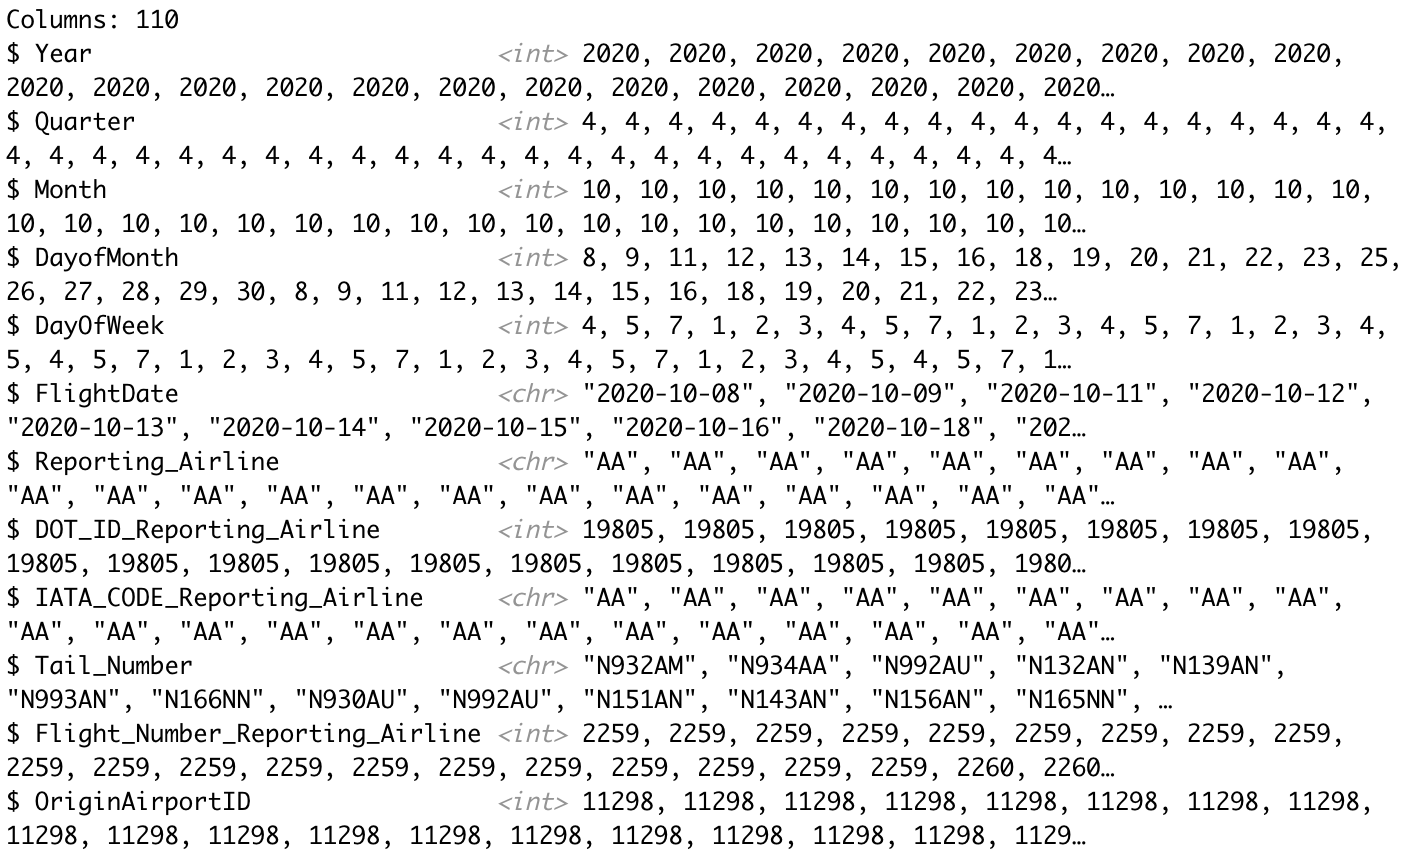
\includegraphics[scale=0.35]{datastru.png} 
\small
\caption{Data frame}
\end{figure}
\end{frame}

\begin{frame}{Data Wrangling}
\begin{figure}
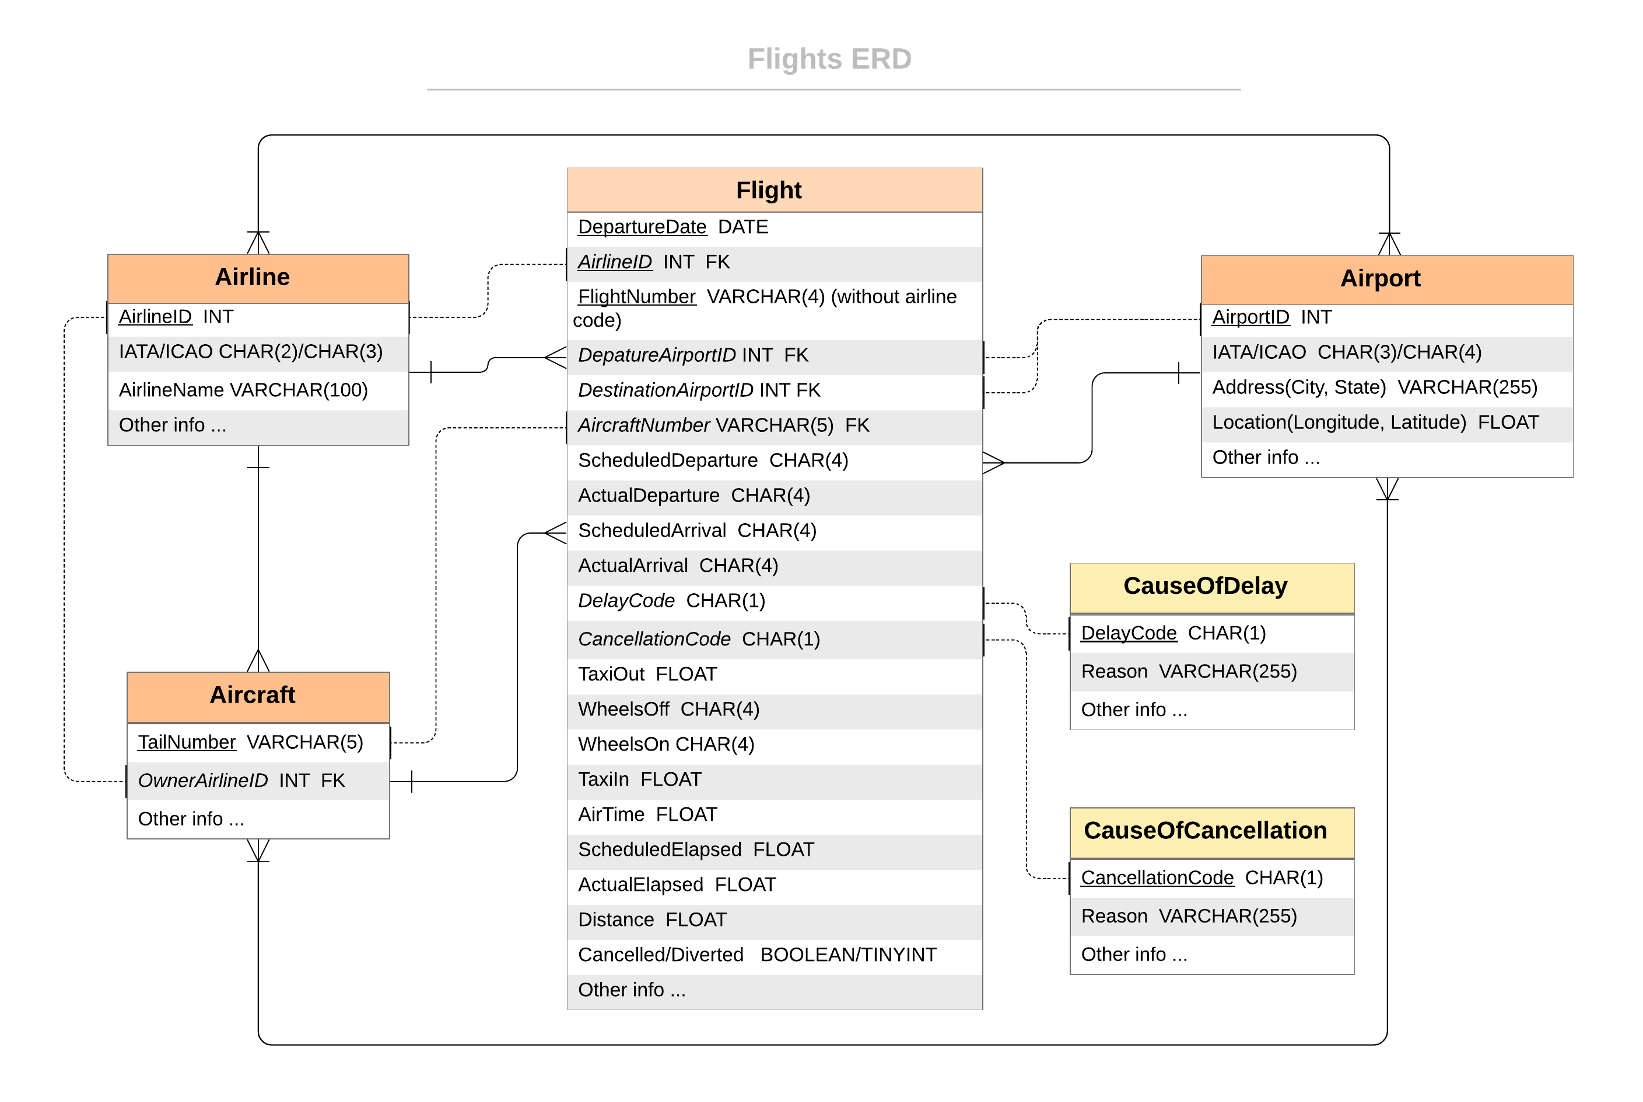
\includegraphics[scale=0.35]{ERD.png} 
\small
\caption{Entity Relation Diagram}
\end{figure}
\end{frame}

\begin{frame}{Interesting Findings}
Pareto principle(20-80 rule): we found top 10\% of airports with the most significant annual number of scheduled flights own more than 94.8\% of flights. Ridiculously, the top 10\% of airlines take up over 97.7\% of all flights.  Monopoly?\\
Indicating large airports and airlines by half-normal plots:\\
\center
\begin{figure}
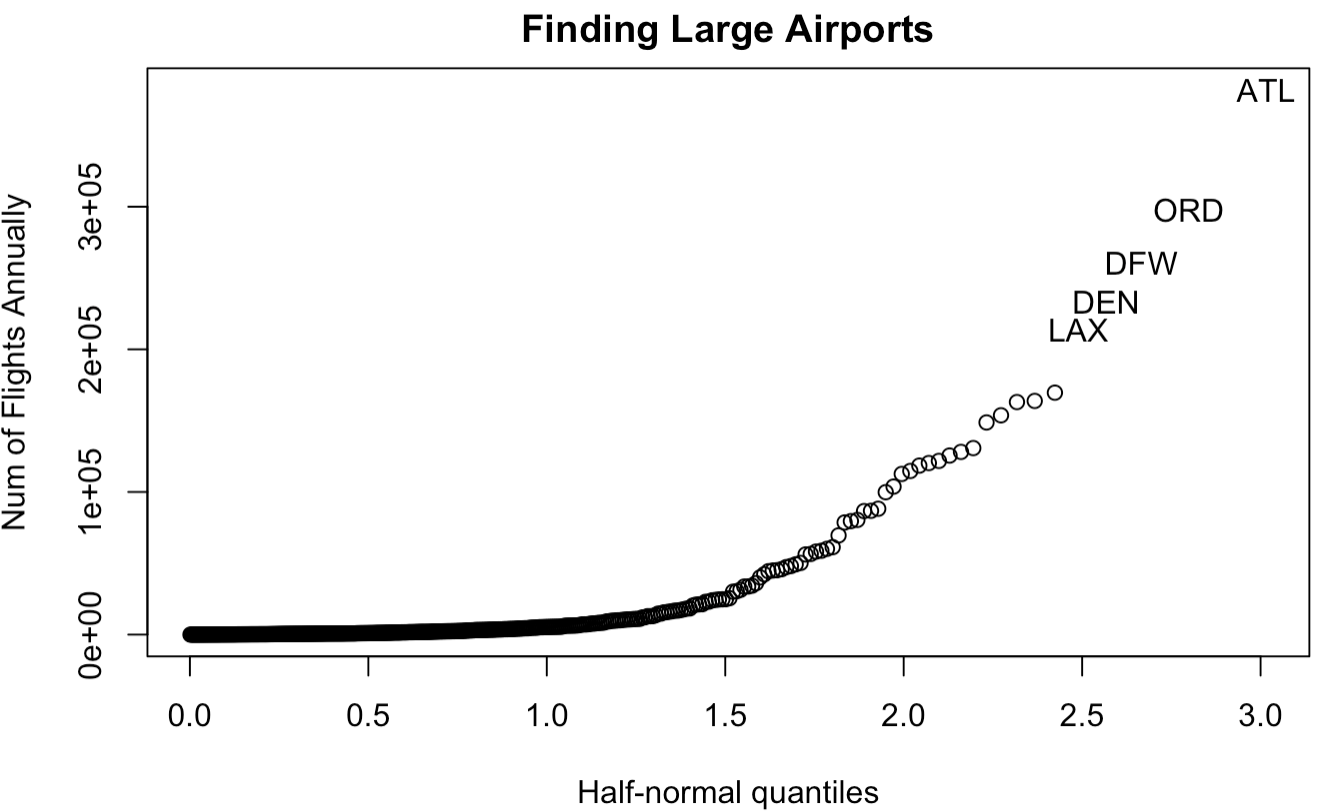
\includegraphics[scale=0.25]{halfnormap.png} 
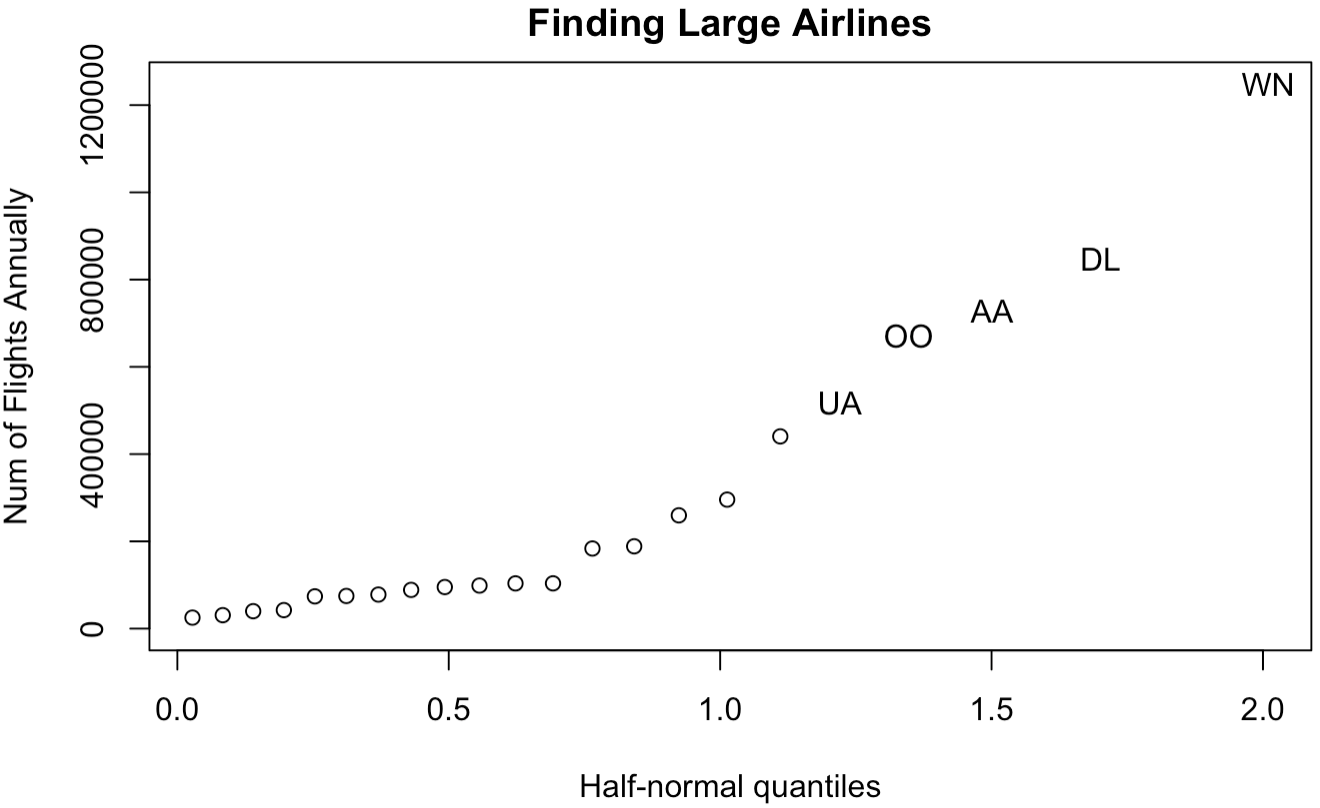
\includegraphics[scale=0.25]{halfnormal.png} 
\small
\caption{Indicating leverages}
\end{figure}
\end{frame}

\begin{frame}{Interesting Findings}
Focusing on number of flights within a day,  we have
\center
\begin{figure}
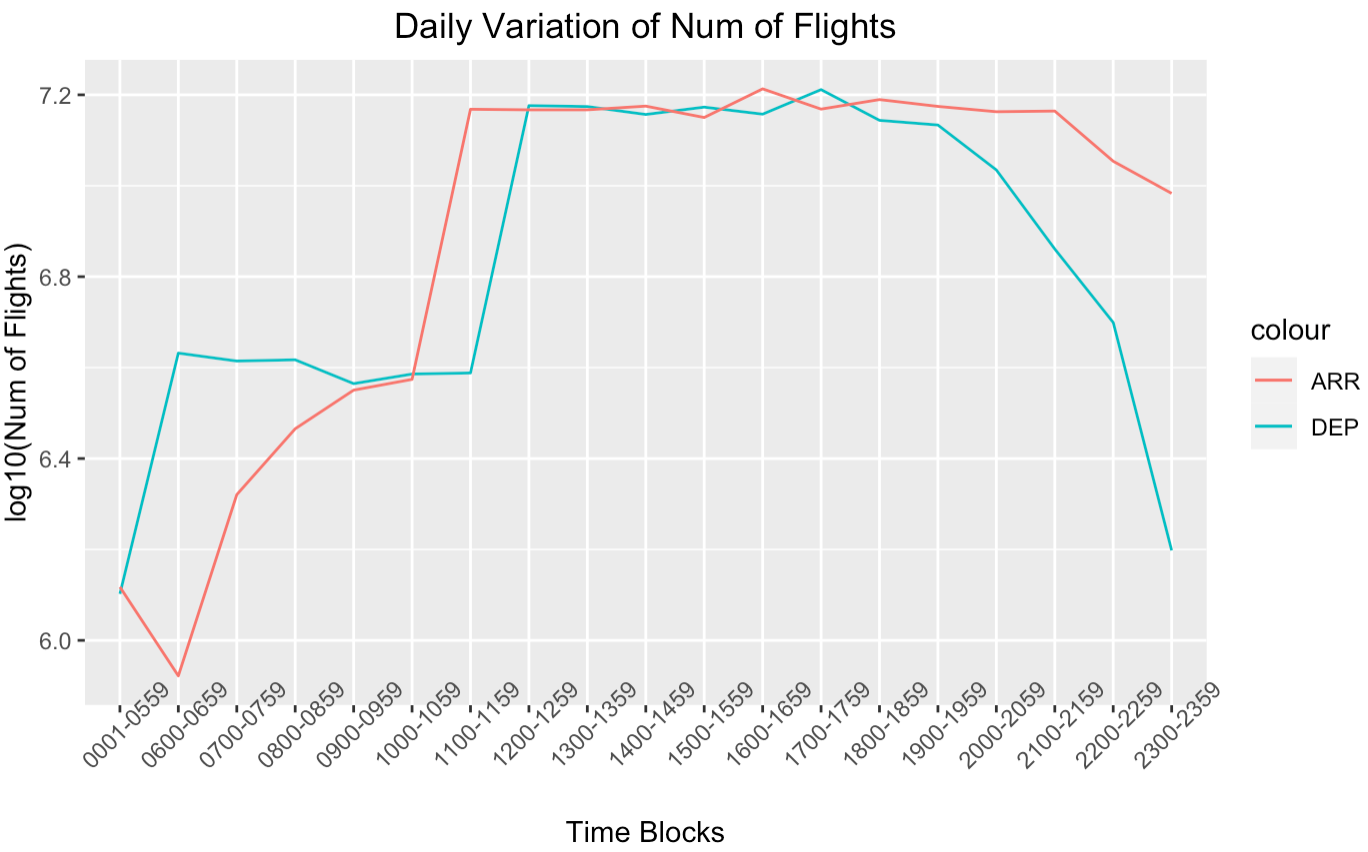
\includegraphics[scale=0.4]{dailyvariation.png} 
\small
\caption{Compare departure and arrival traffic flows by time block}
\end{figure}
\end{frame}

\begin{frame}{Interesting Findings}
\begin{itemize}
\item Mondays, Thursdays and Fridays have the most delays.
\item June, July and August have the most delays.
\item Both airport locations and flight routes are denser in the east coast.
\end{itemize}
\center
\begin{figure}
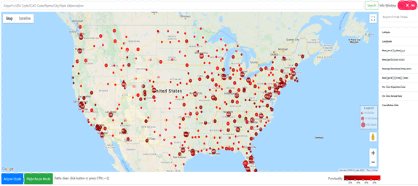
\includegraphics[scale=0.8]{airportdist.png} 
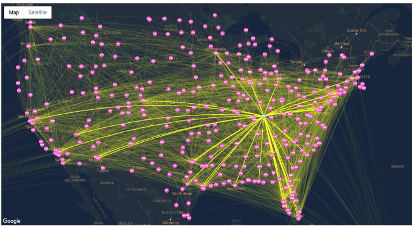
\includegraphics[scale=0.7]{interconn.png} 
\small
\caption{Distribution of airports and their interconnectivity}
\end{figure}
\end{frame}

\begin{frame}{Interesting Findings}
Anomaly Detections
\center
\begin{figure}
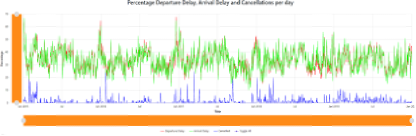
\includegraphics[scale=1]{longseries.png} \\
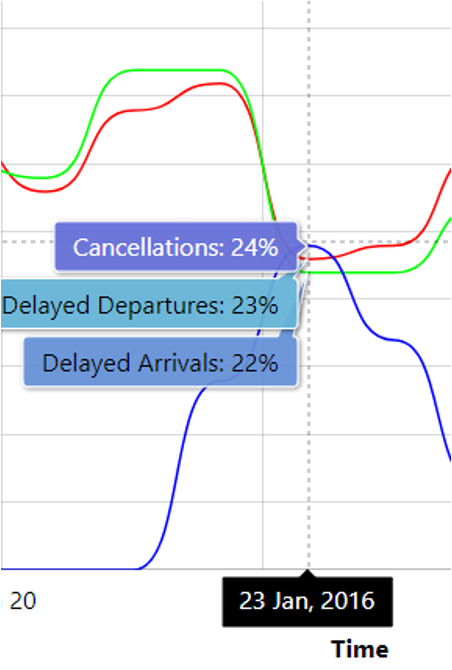
\includegraphics[scale=0.3]{incidentplot.png} 
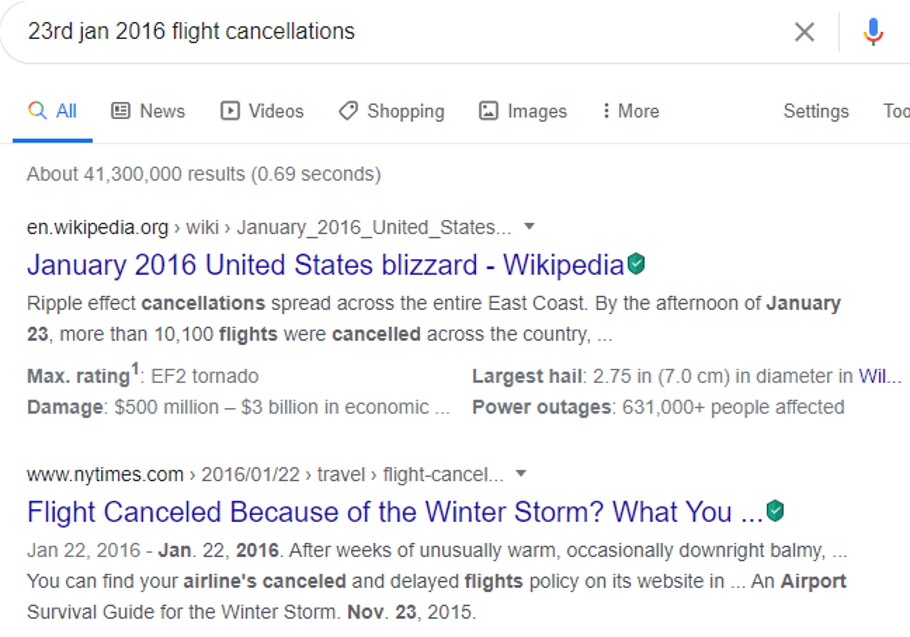
\includegraphics[scale=0.3]{googleincident.png}
\small
\caption{Find an Incident from interactive series}
\end{figure}
\end{frame}

\begin{frame}{Overall Series}
\center
\begin{figure}
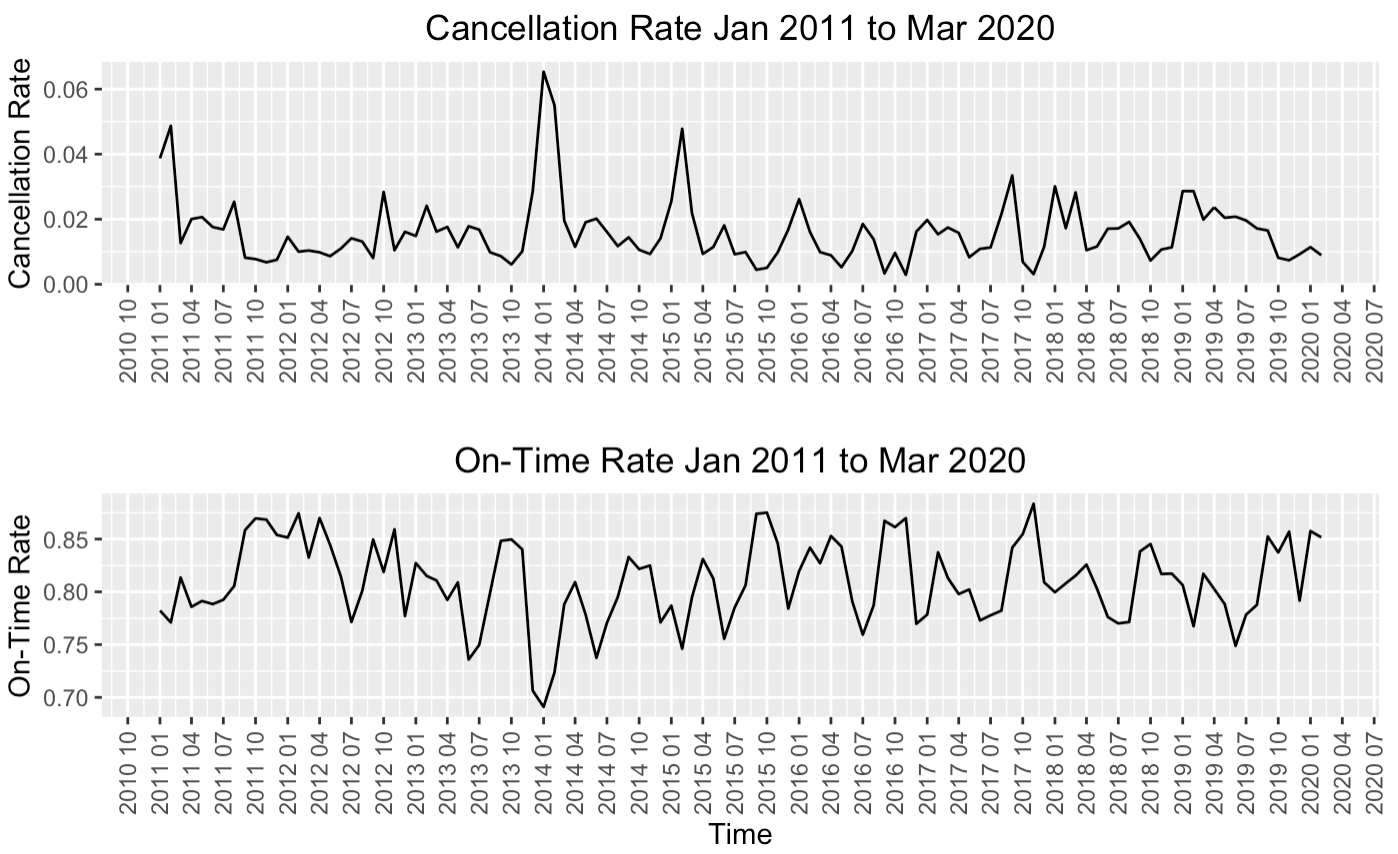
\includegraphics[scale=0.4]{cancelvsontime.png}
\caption{Compare monthly CR and OTR.  Note the scale!}
\end{figure}
\end{frame}

\begin{frame}{Overall Series}
\center
\begin{figure}
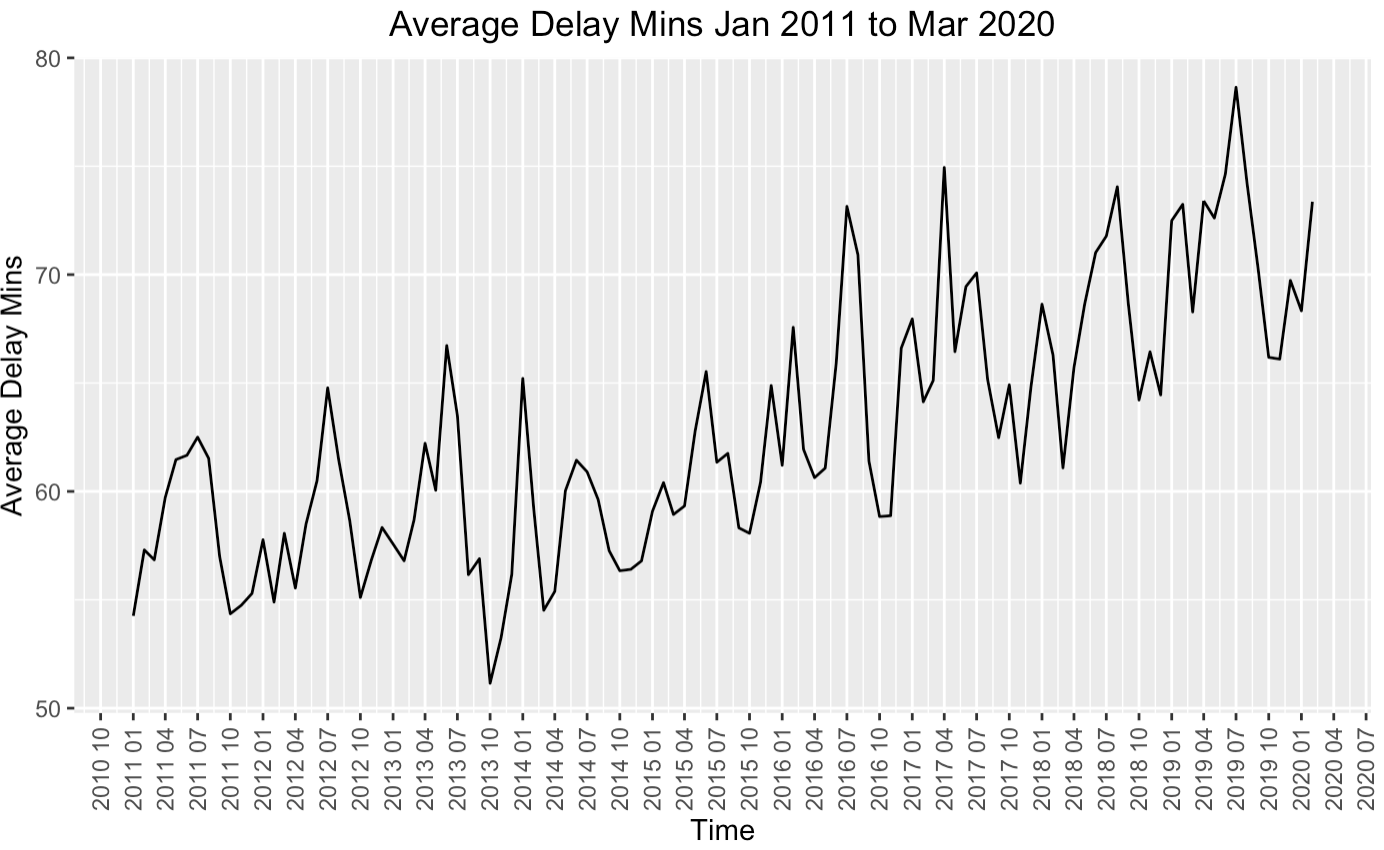
\includegraphics[scale=0.4]{avgdelaymin.png}
\caption{Monthly ADM.  Suggest a Moving Average model}
\end{figure}
\end{frame}

\begin{frame} {Series Decomposition}

\center
\begin{figure}
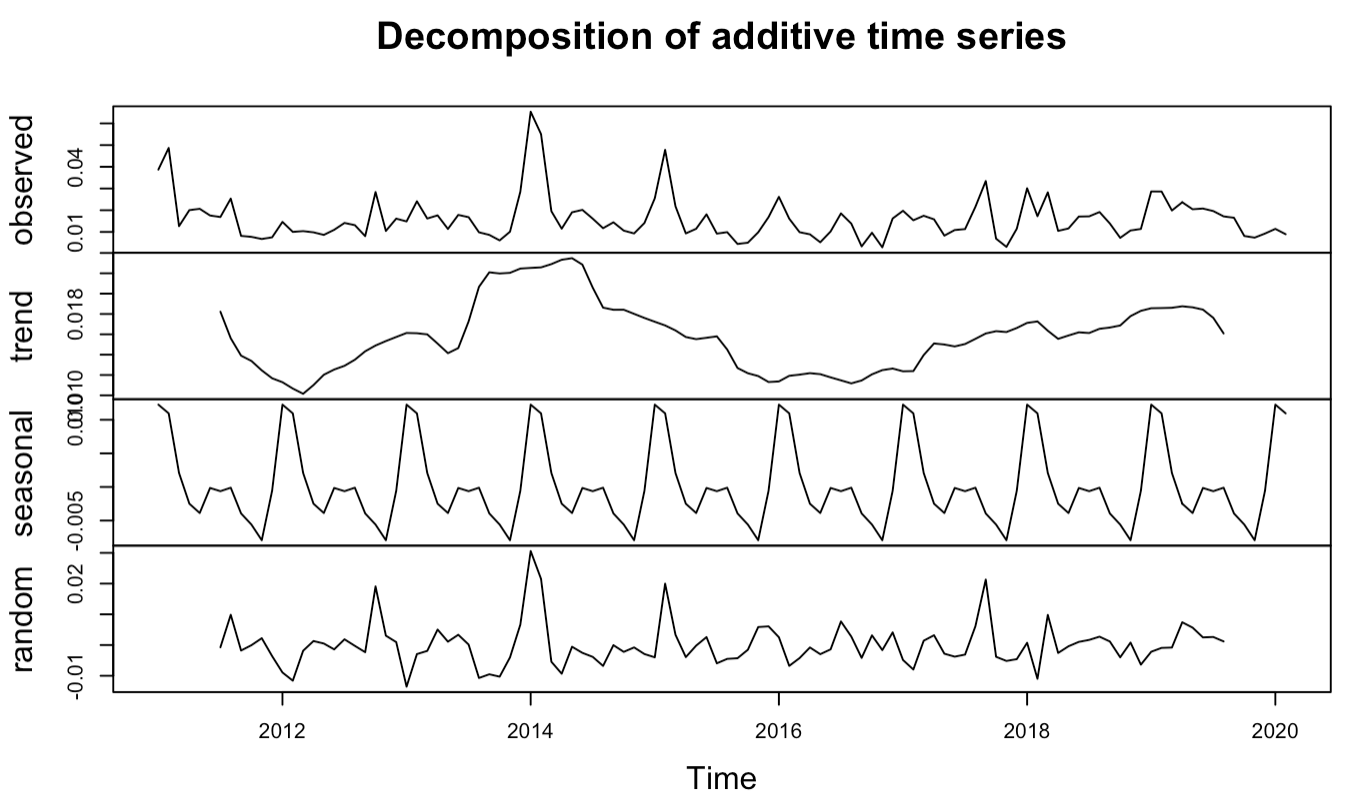
\includegraphics[scale=0.2]{decompcancel.png} 
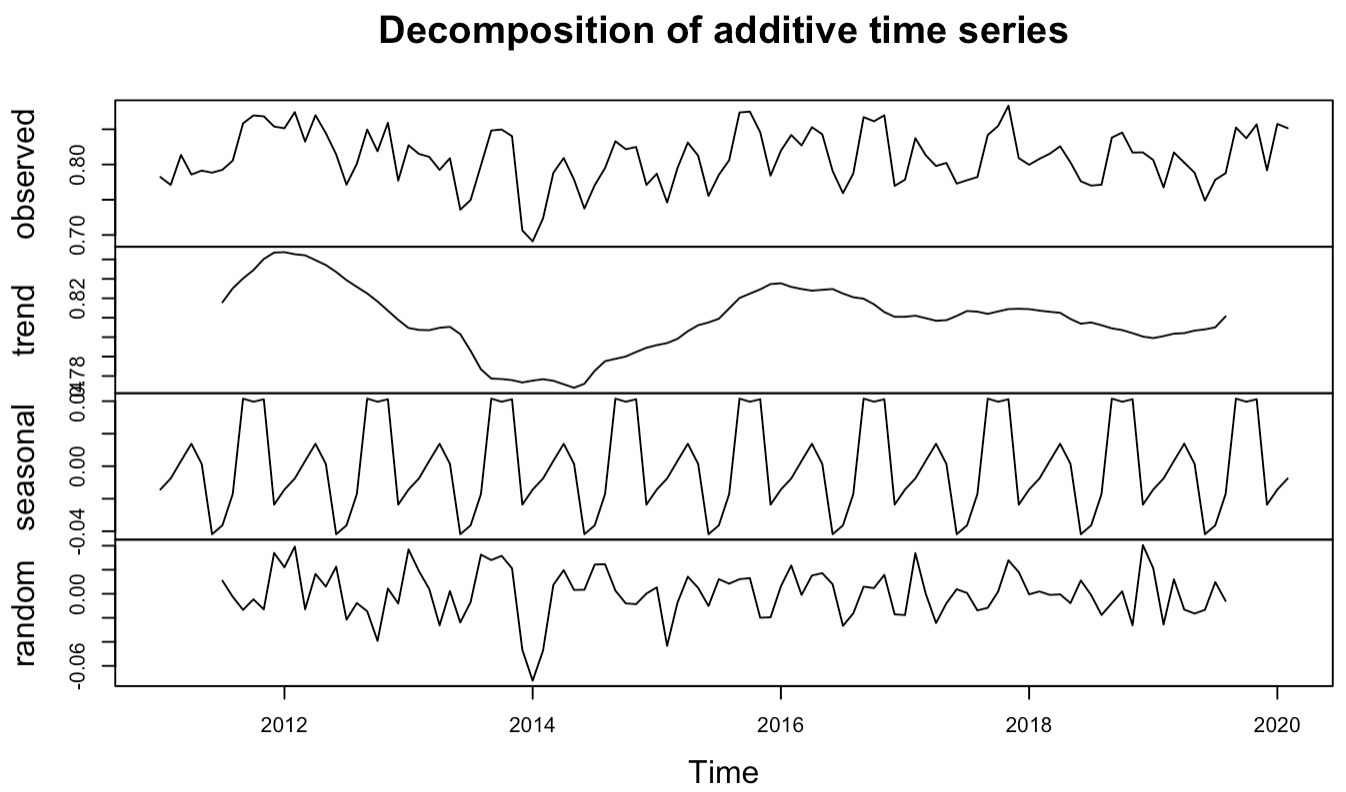
\includegraphics[scale=0.2]{decompontime.png} \\
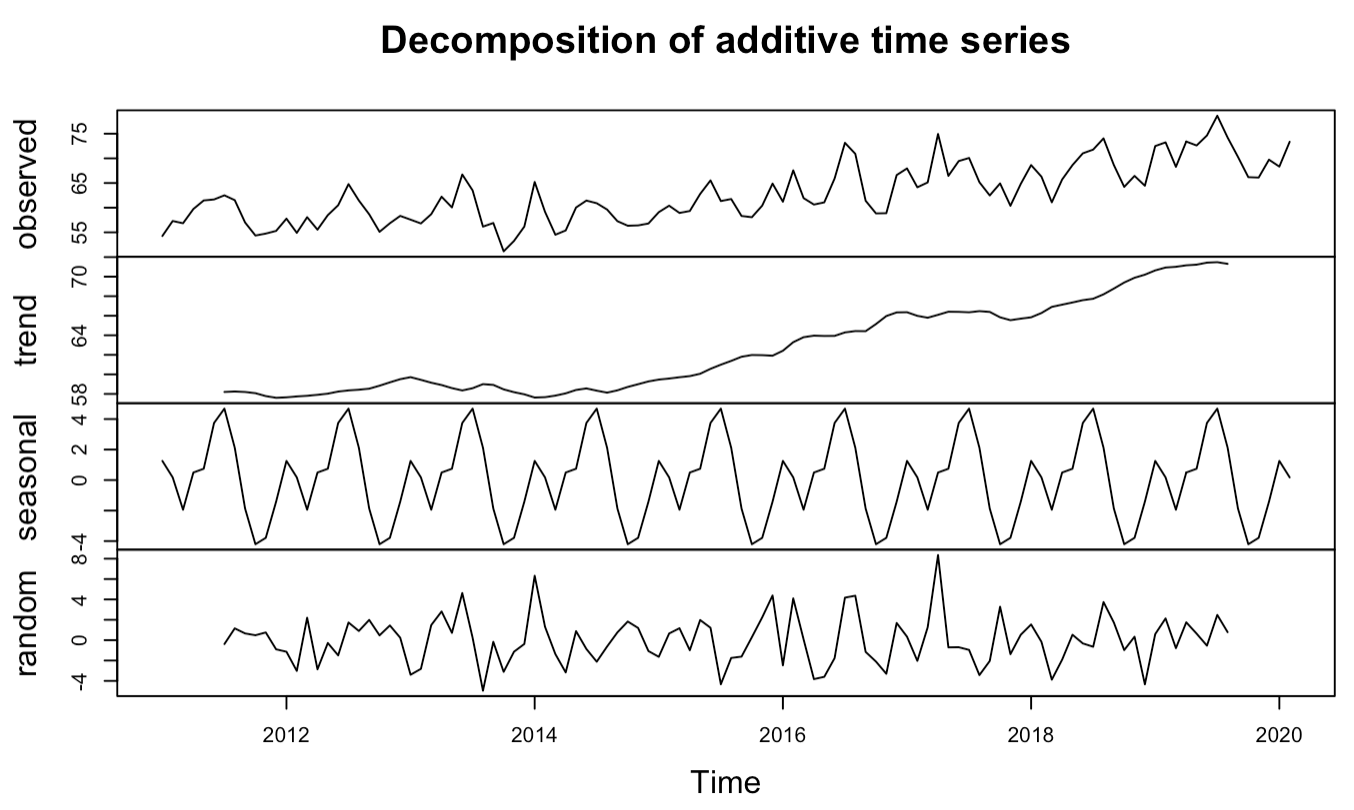
\includegraphics[scale=0.2]{decompadm.png} 
\caption{Decomposition of 3 series}
\end{figure}
\end{frame}

\begin{frame} {Essentials of Seasonal ARIMA Model}
Assume we have a seasonal time series $\{Y_t\}^T_{t=1}$, which is fitted by a seasonal model ARIMA$(p,d,q)(P,D,Q)_m$,  where $(p,d,q)$ refers to non-seasonal part, $(P,D,Q)$ refers to seasonal one and $m=$ the number of observations each year. \\
Define the seasonal differencing: $$(1-B^S)Y_t=Y_t-Y_{t-S}$$ and non-seasonal differencing $$(1-B)Y_t=Y_t-Y_{t-1}$$ for the trend.
So, we can examine the model through $$(1-B^{12})(1-B)Y_t=(Y_t-Y_{t-{12}})-(Y_t-Y_{t-1})$$.
\end{frame}

\begin{frame} {Stationarity Testing}
Evidently, there is a seasonal pattern, which indicates a nonstationarity before seasonal differencing.
\begin{figure}
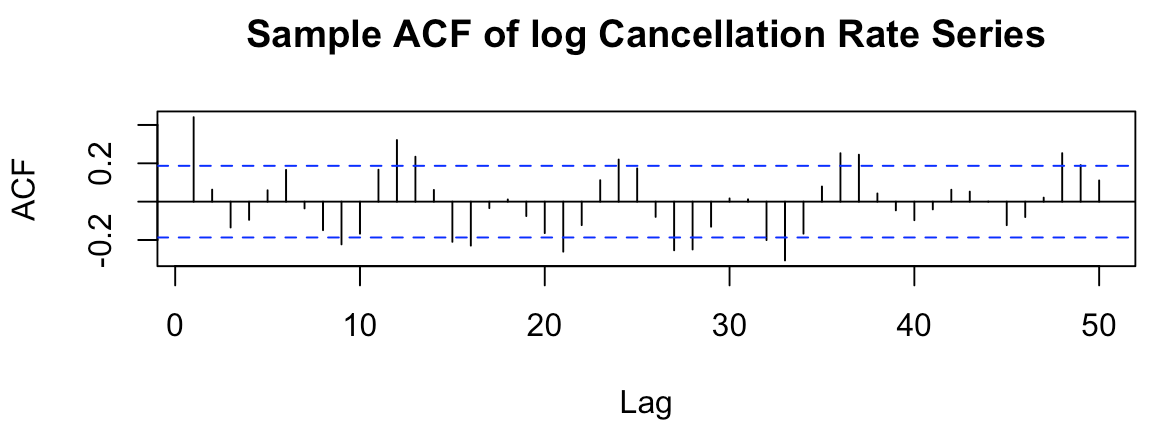
\includegraphics[scale=0.25]{CRacf.png} 
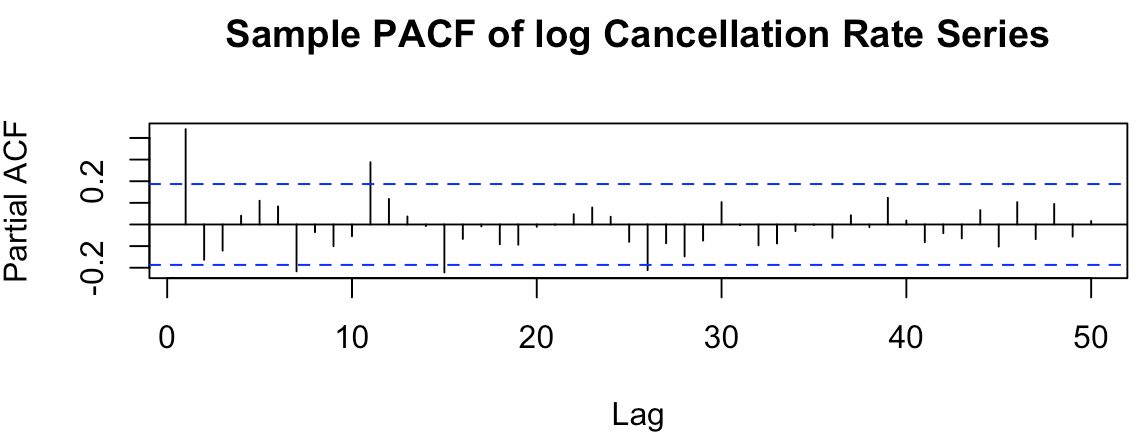
\includegraphics[scale=0.25]{CRpacf.png} \\
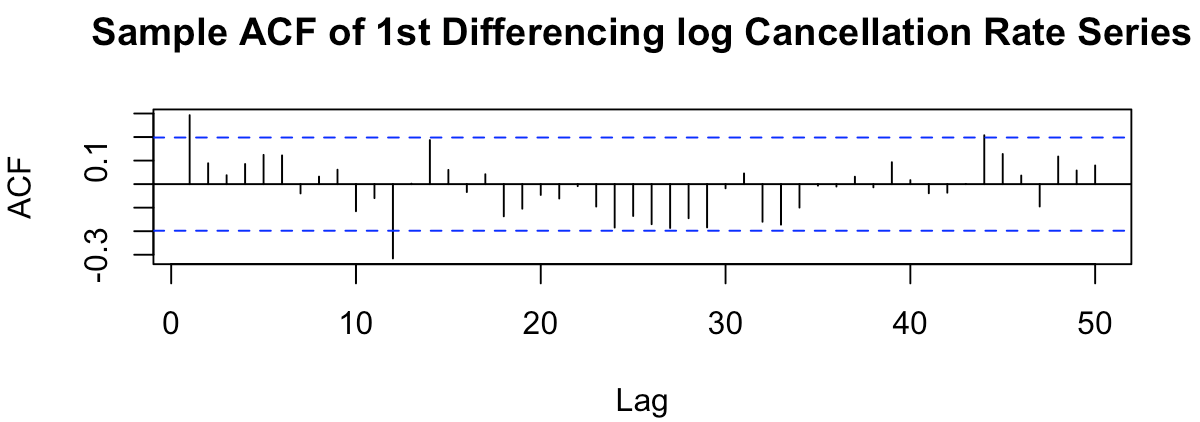
\includegraphics[scale=0.25]{CRacf1st.png} 
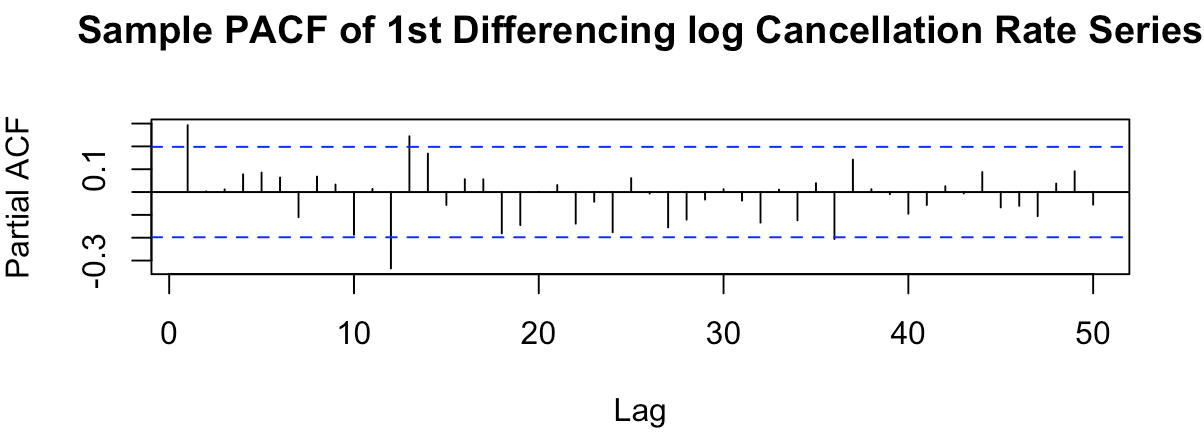
\includegraphics[scale=0.25]{CRpacf1st.png} 
{\center \small Nonseasonal behavior: The PACF of 1st diff shows a clear spike at lag 1 and not much else until lag 36.  Try AR(2) or AR(3).  Seasonal behavior: In the PACF,  there’s a cluster of spikes around lag 12 and then not much else.  Try SAR(1). }
\caption{ACF plots and PACF plots of CR series}
\end{figure}
\end{frame}

\begin{frame} {Stationarity Testing}
\begin{figure}
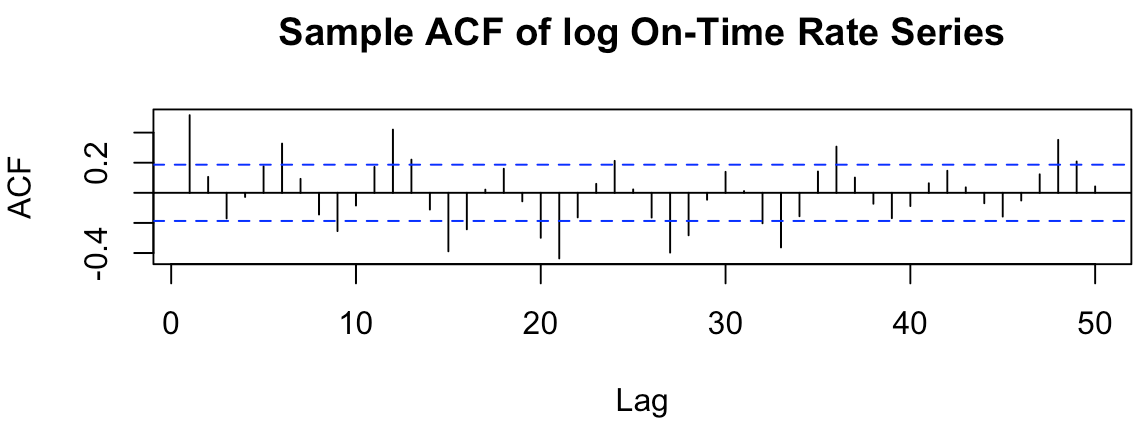
\includegraphics[scale=0.25]{OTRacf.png} 
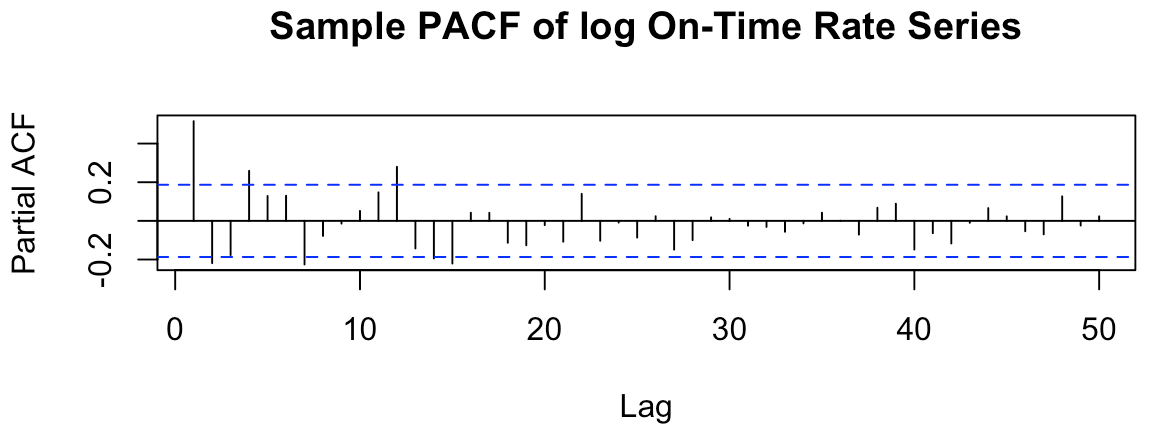
\includegraphics[scale=0.25]{OTRpacf.png} \\
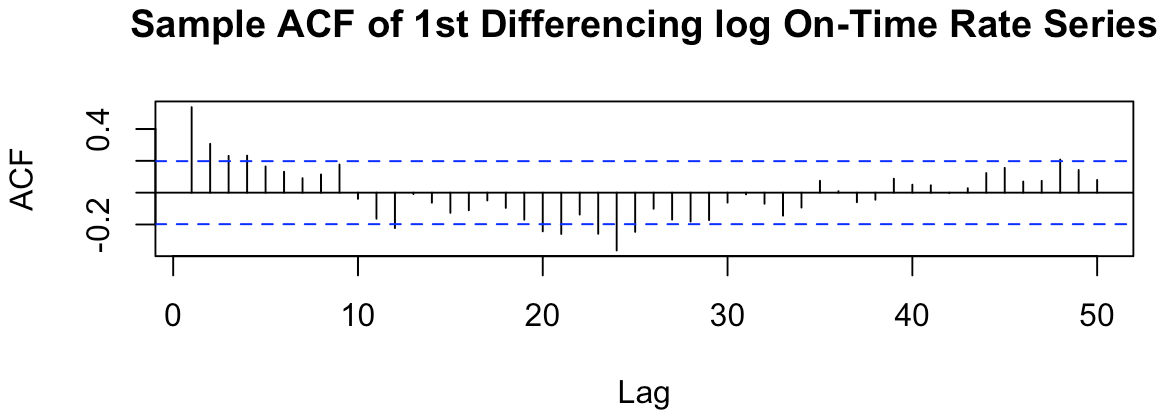
\includegraphics[scale=0.25]{OTRacf1st.png} 
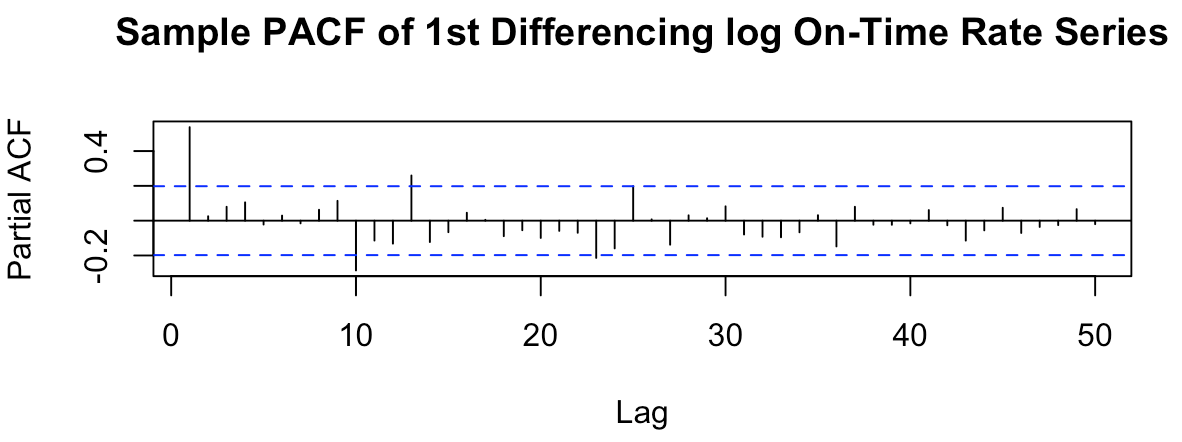
\includegraphics[scale=0.25]{OTRpacf1st.png} 
{\center \small Nonseasonal behavior: The PACF of 1st diff shows a clear spike at lag 1 and not much else until lag 23.  Try AR(1).  Seasonal behavior: In the PACF of 1st diff,  there’s a cluster of spikes around lag 12,24 and then not much else.  Try from SAR(2,0) to SARI(2,3), etc. }
\caption{ACF plots and PACF plots of OTR series}
\end{figure}
\end{frame}

\begin{frame} {Stationarity Testing}
\begin{figure}
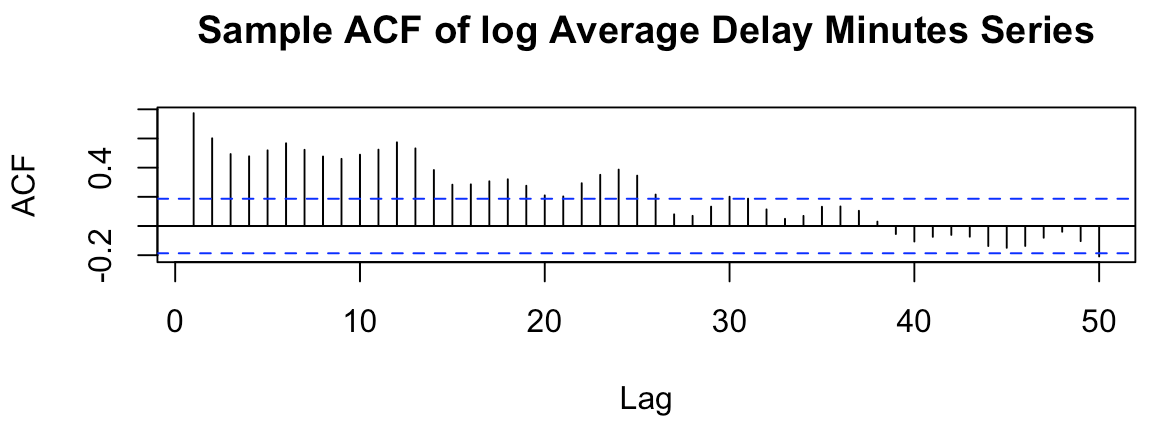
\includegraphics[scale=0.27]{ADMacf.png} 
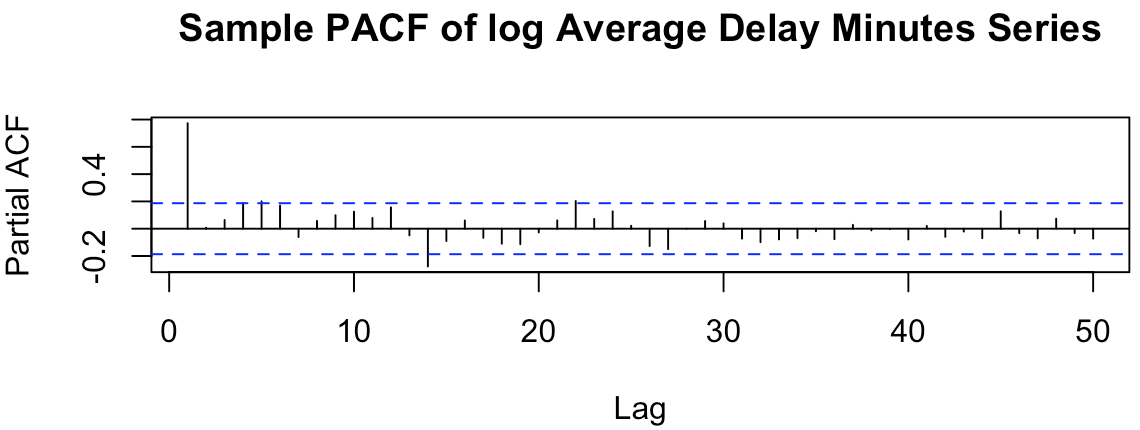
\includegraphics[scale=0.27]{ADMpacf.png} \\
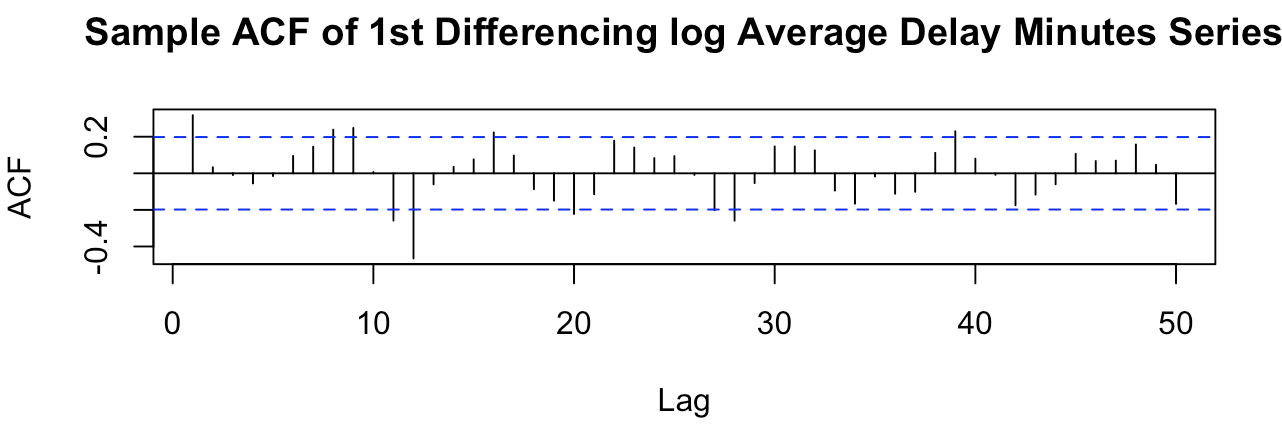
\includegraphics[scale=0.25]{ADMacf1st.png} 
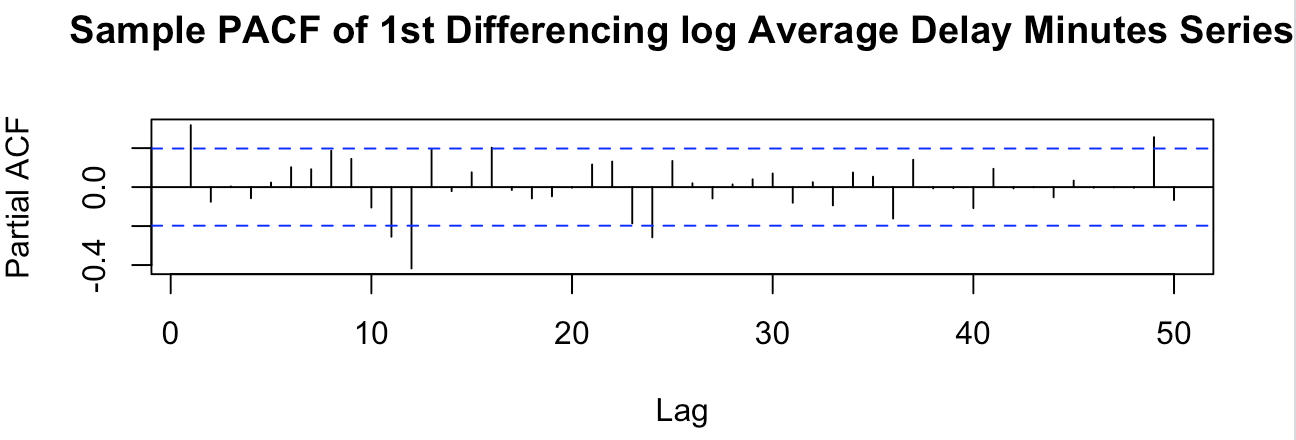
\includegraphics[scale=0.25]{ADMpacf1st.png} 
{\center \small Nonseasonal behavior: The ACF of 1st diff shows spikes at lag 12, and not much else until lag 28.  Try from MA(2) to IMA(3,2).  Seasonal behavior: In the ACF of 1st diff,  there’s a cluster of spikes around lag 12,28 and then not much else.  Try MA(2).}
\caption{ACF plots and PACF plots of ADM series}
\end{figure}
\end{frame}


\begin{frame} {Stationarity Testing}
The augmented Dickey-Fuller (ADF) test statistic is the t-statistic of the estimated coefficient of $\alpha$ from the method of least squares regression.  \footnote{SHUMWAY, R. H., \& STOFFER, D. S. (2006). Time series analysis and its applications: with R examples. New York,  Springer.} 
{ \small Lag order = 12, \\  p-value of log CR series = 0.6401,  \\ p-value of log OTR series = 0.6764,  \\ p-value of log ADM series = 0.6241 }
\end{frame}

\begin{frame} {Model Specification}
Suppose a ARIMA($p,d,q$) model, where $p,q$ are determined by minimum AIC(find a good model to predict) and BIC(find a best fit to the data).\\
We find 
\begin{description}[Other description]
\item[CR series] ARIMA(2,0,0)$\times$(1,0,0)[12]\\ with AIC=-725.24,  BIC=-711.74 and $\sigma^2<1e-4$.
\item[OTR series] ARIMA(1,0,0)$\times$(2,1,0)[12]\\  with AIC=-411.26,  BIC=-400.92 and $\sigma^2<1e-3$.
\item[ADM series] ARIMA(0,1,2)$\times$(0,0,2)[12]\\ with AIC=574  BIC=590.15 and $\sigma^2=10.36$.
\end{description}
\end{frame}

\begin{frame} {Residual Analysis}
\begin{figure}
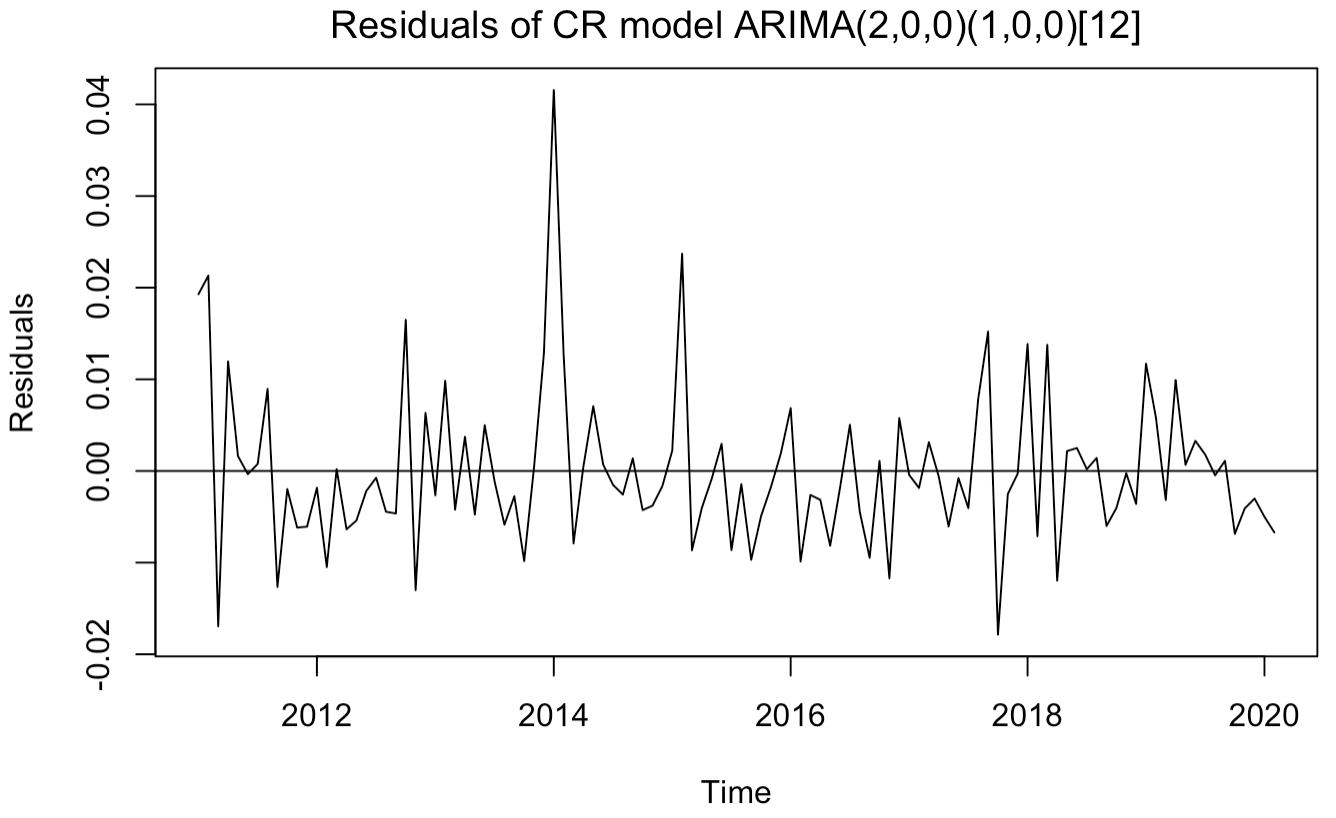
\includegraphics[scale=0.23]{CRresid.png} 
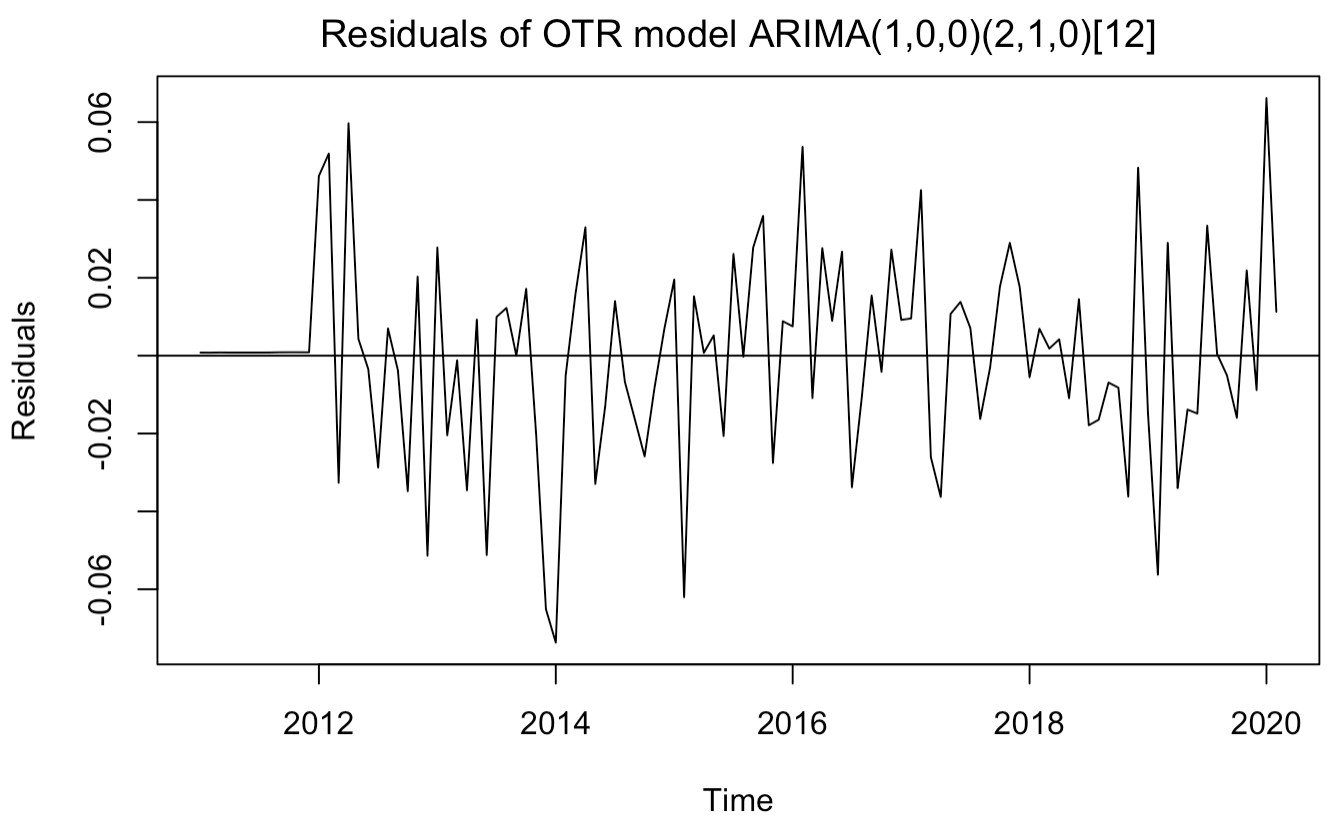
\includegraphics[scale=0.23]{OTRresid.png} \\
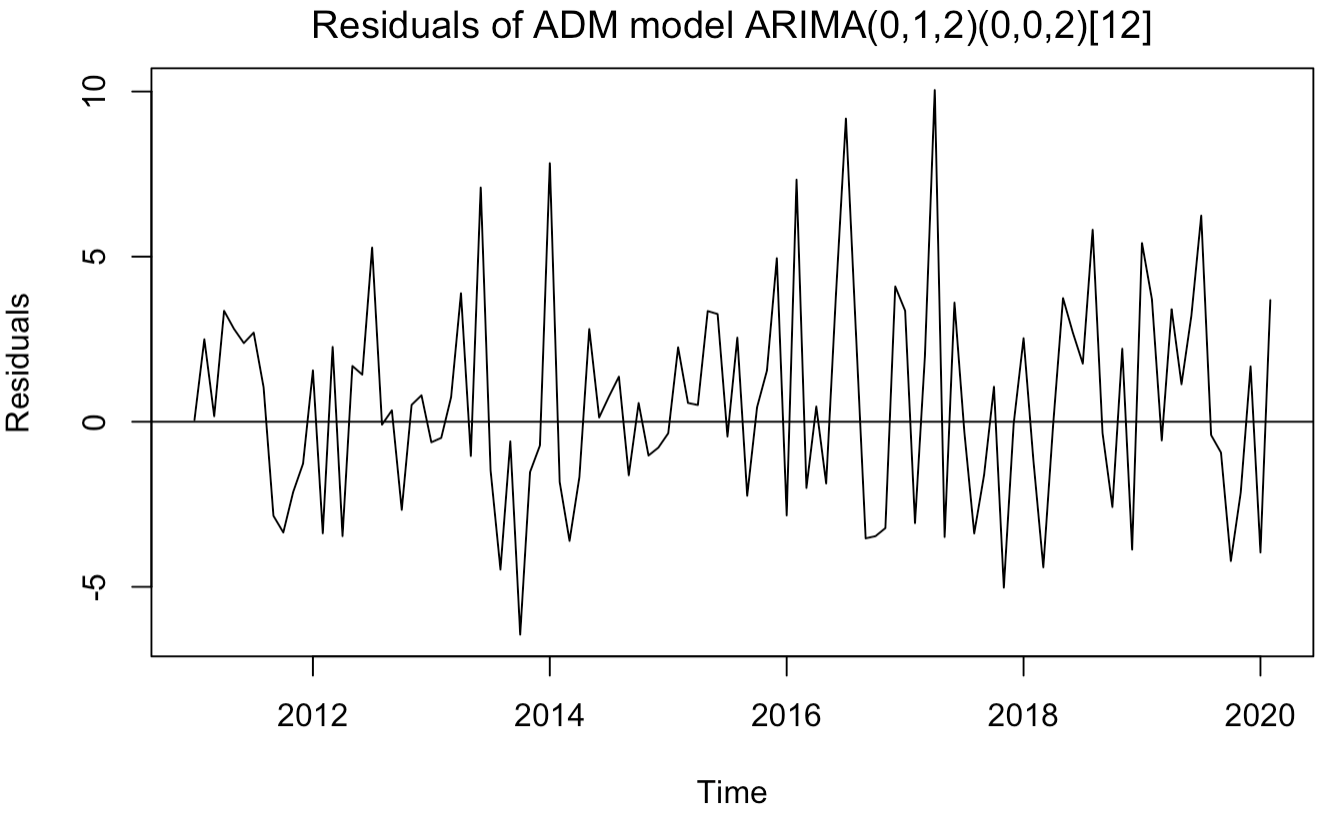
\includegraphics[scale=0.23]{ADMresid.png} 
\caption{Residual Plots}
\end{figure}
\end{frame}

\begin{frame} {Ljung-Box Test and Normality Assumption}
According to Ljung-Box Test and Shapiro-Wilk normality test, we have p-values of three residuals.
\begin{description}[Other description]
\item[CR series] LB:0.5767, SW: 9.682e-07, reject normality.
\item[OTR series] LB:0.1702, SW:0.1446.
\item[ADM series] LB:0.8637, SW:0.1287.
\end{description}
\end{frame}

\begin{frame} {Forecasting}
What if no pandemic,...
\begin{figure}
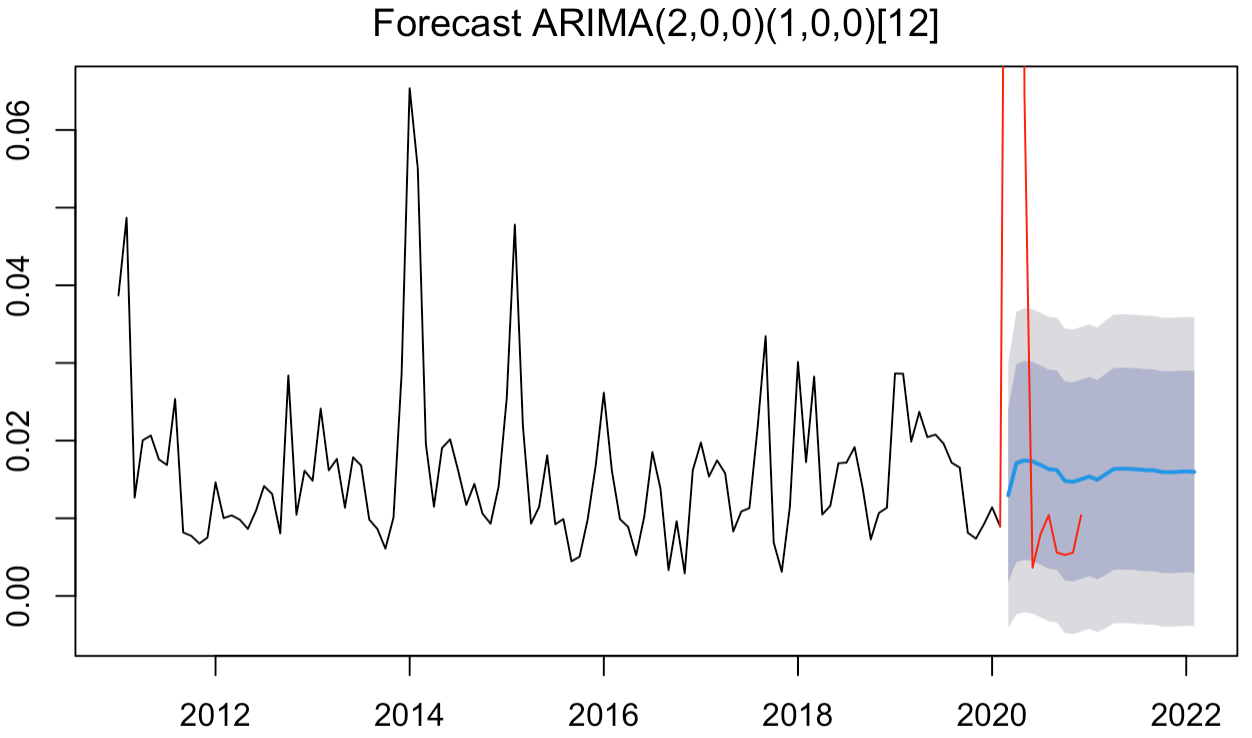
\includegraphics[scale=0.23]{CRforecast.png} 
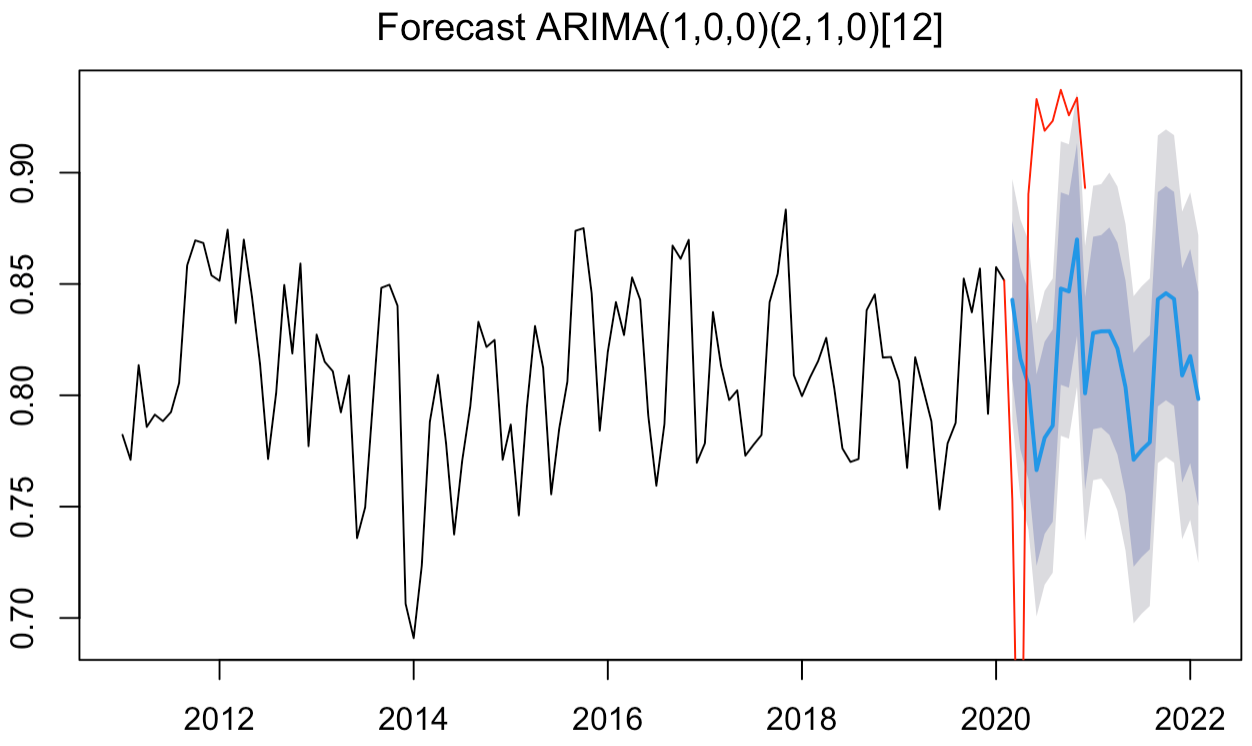
\includegraphics[scale=0.23]{OTRforecast.png} \\
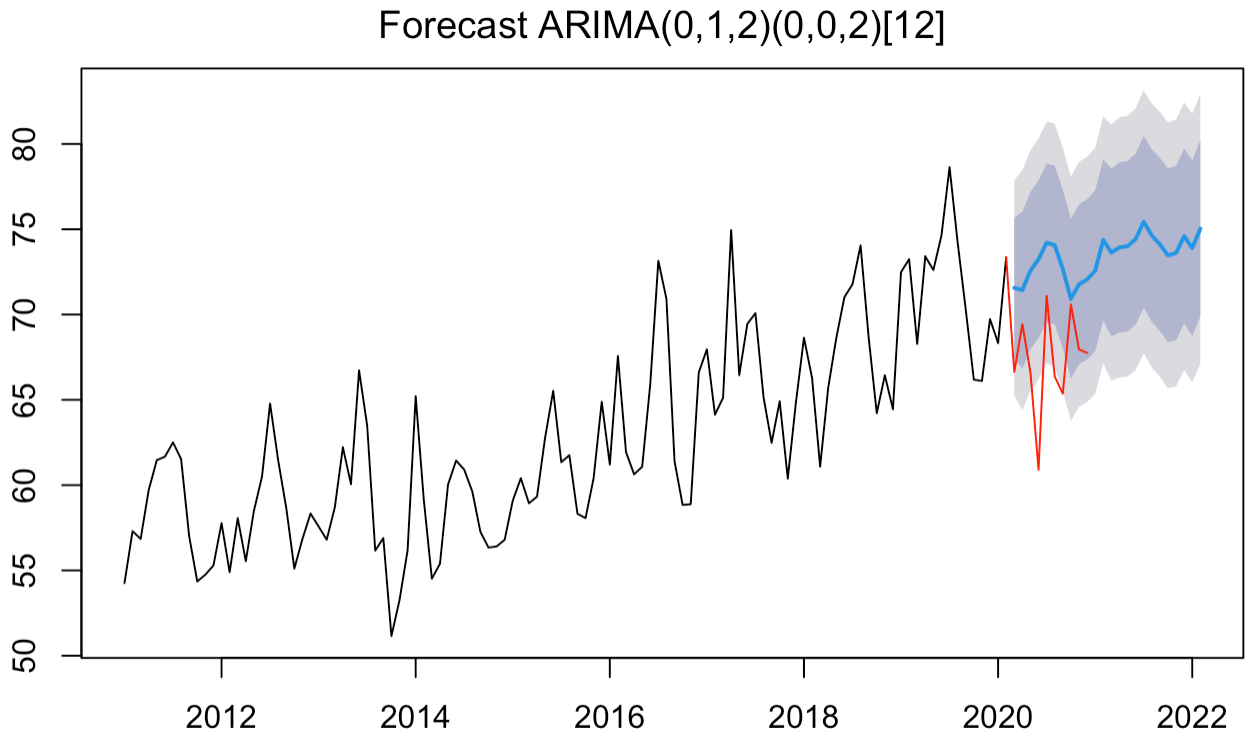
\includegraphics[scale=0.23]{ADMforecast.png} 
\caption{Forecasting Plots}
\end{figure}
\end{frame}

\begin{frame} {Forecasting}
The series after pandemic: CR and OTR model: replace March-April 2020 with the past average; ADM model: fit a new model ARIMA(1,1,0)(0,1,0)[12] from recent 2 years data.
\begin{figure}
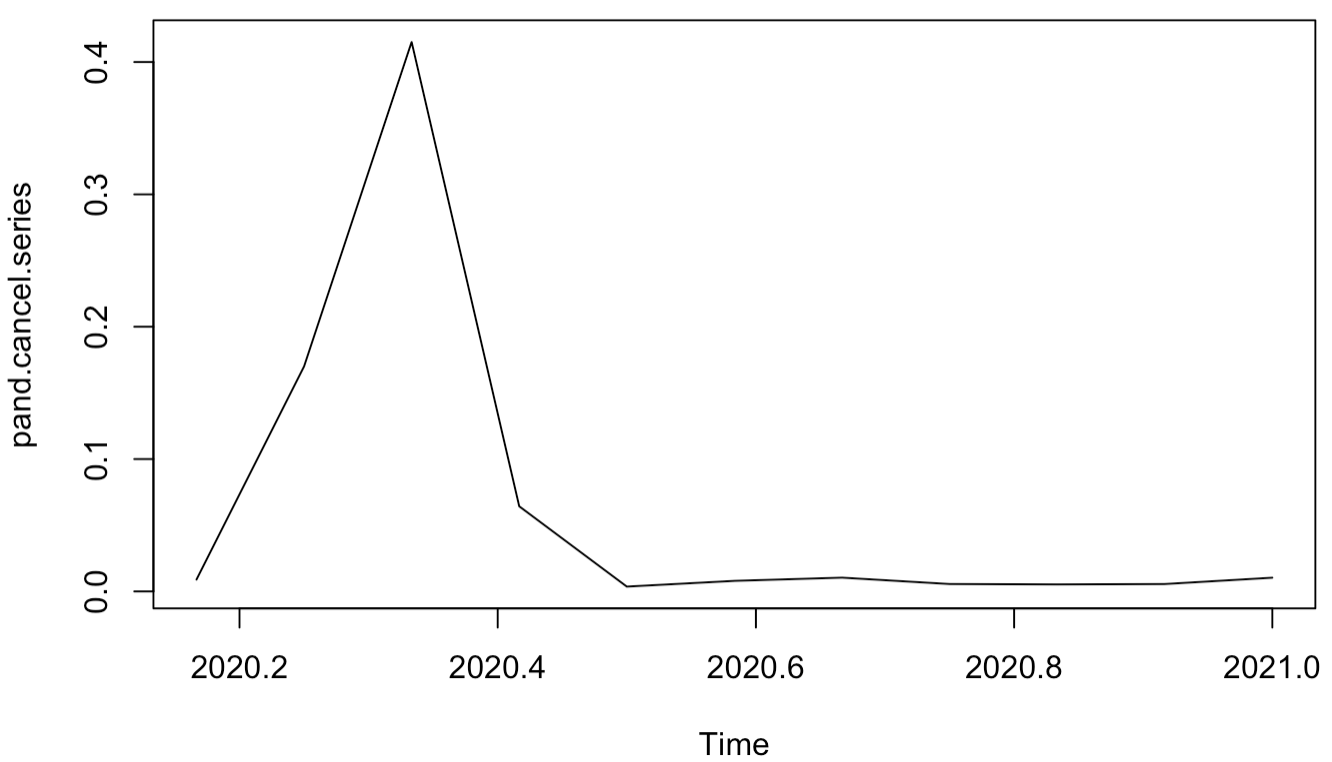
\includegraphics[scale=0.23]{CRpand.png} 
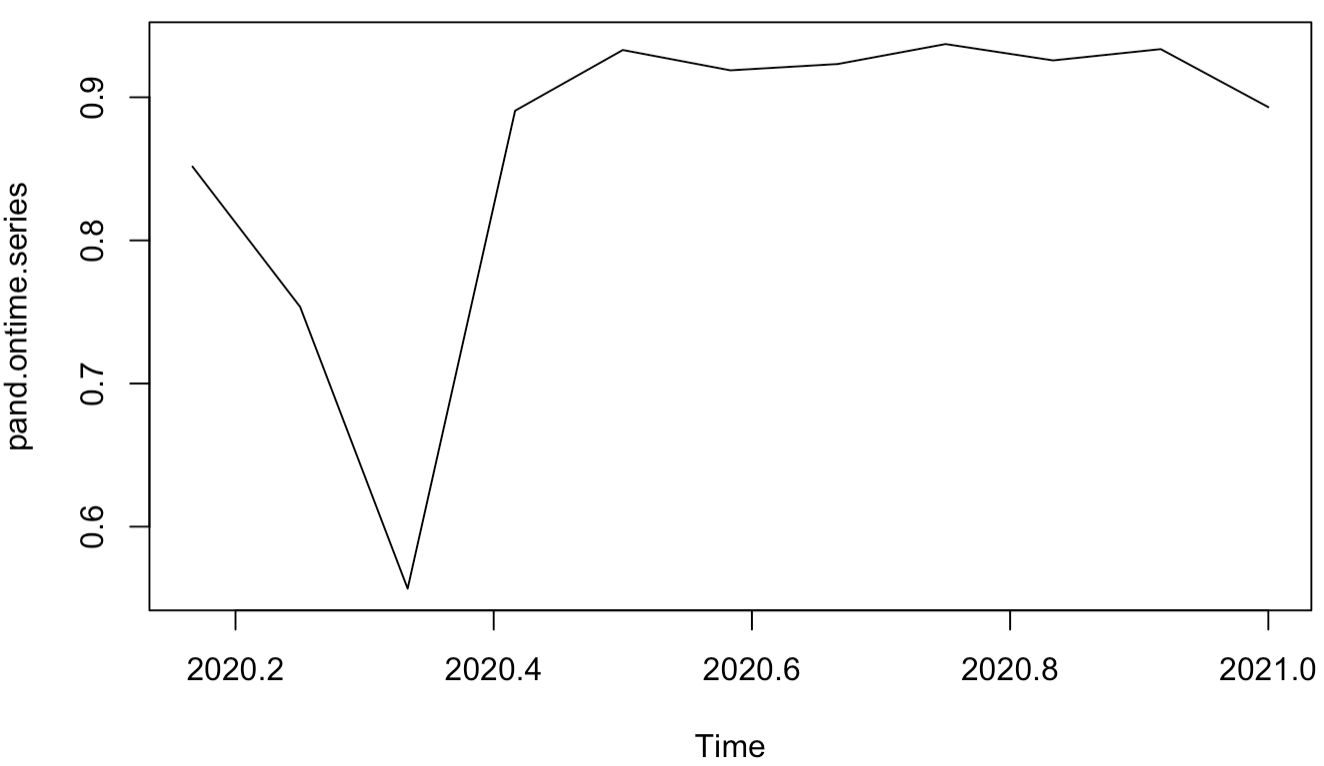
\includegraphics[scale=0.23]{OTRpand.png} \\
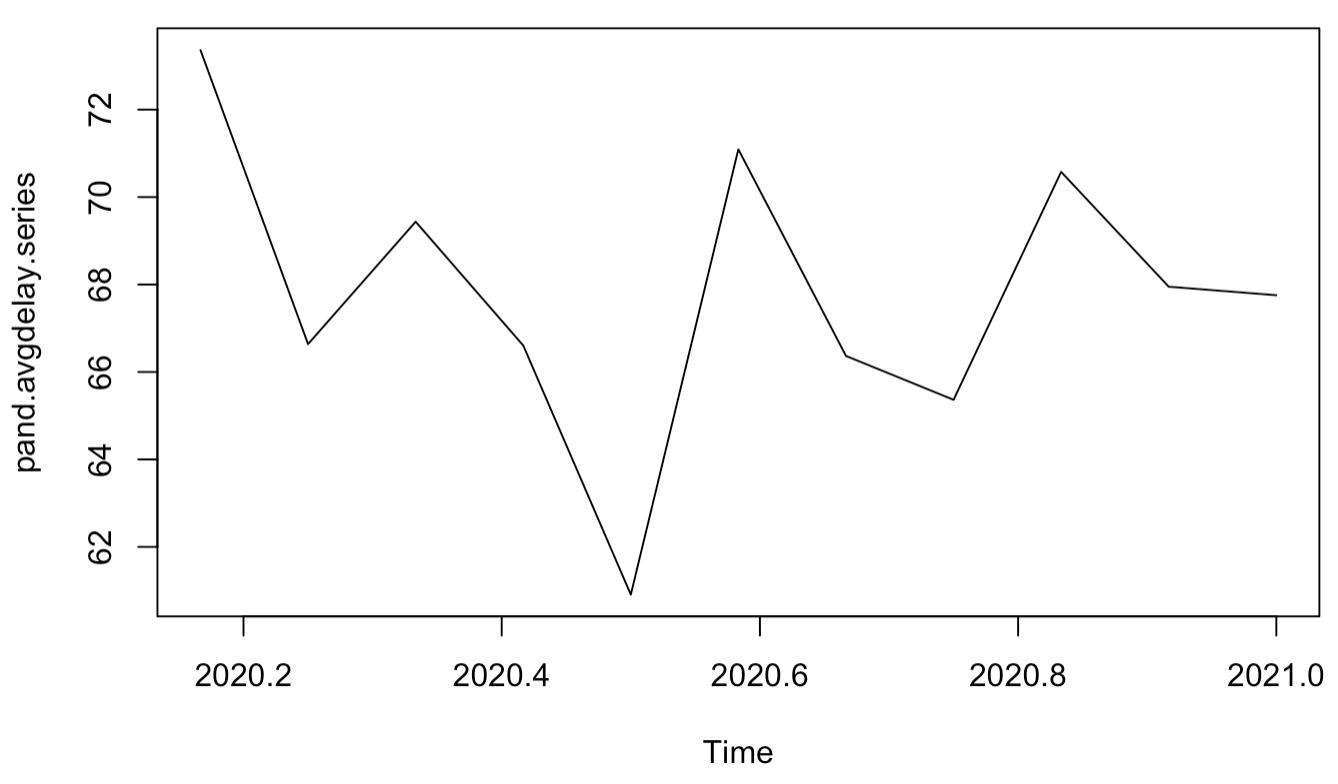
\includegraphics[scale=0.23]{ADMpand.png} 
\caption{Forecasting Plots}
\end{figure}
\end{frame}

\begin{frame} {Forecasting and Verification}
Given 5 more months of data, we have
\begin{figure}
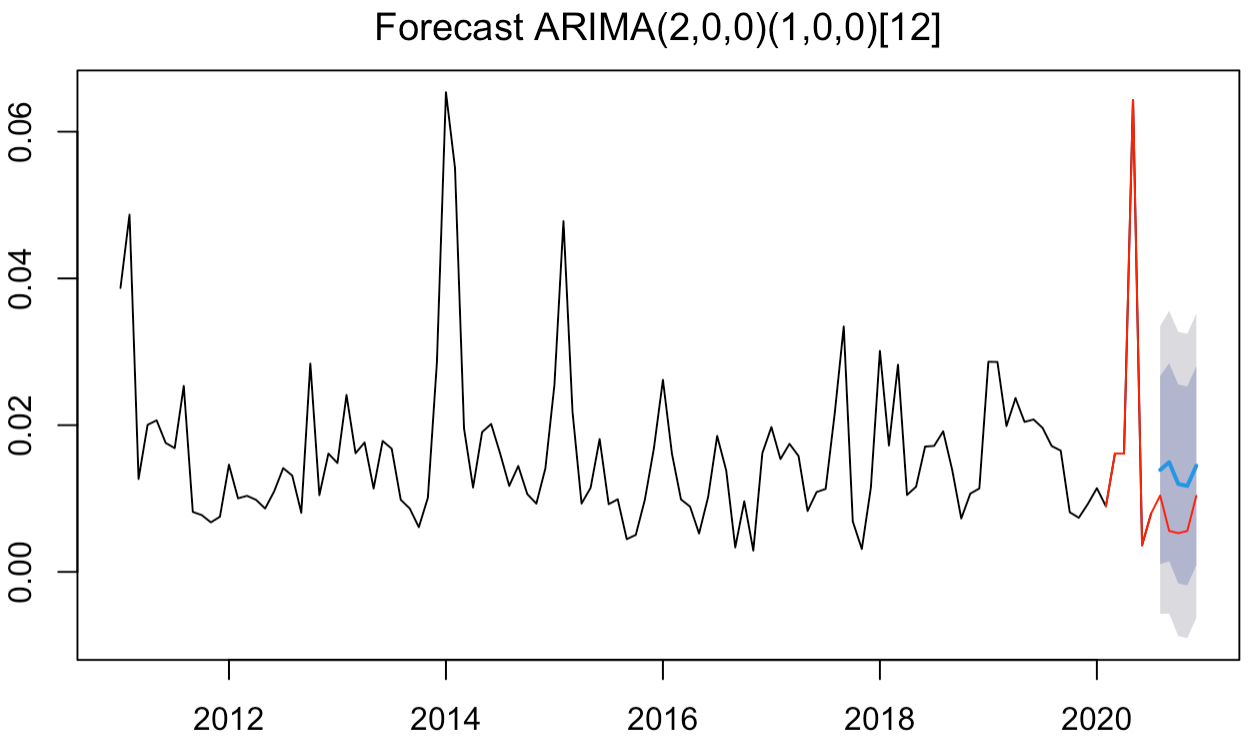
\includegraphics[scale=0.23]{CRpred.png} 
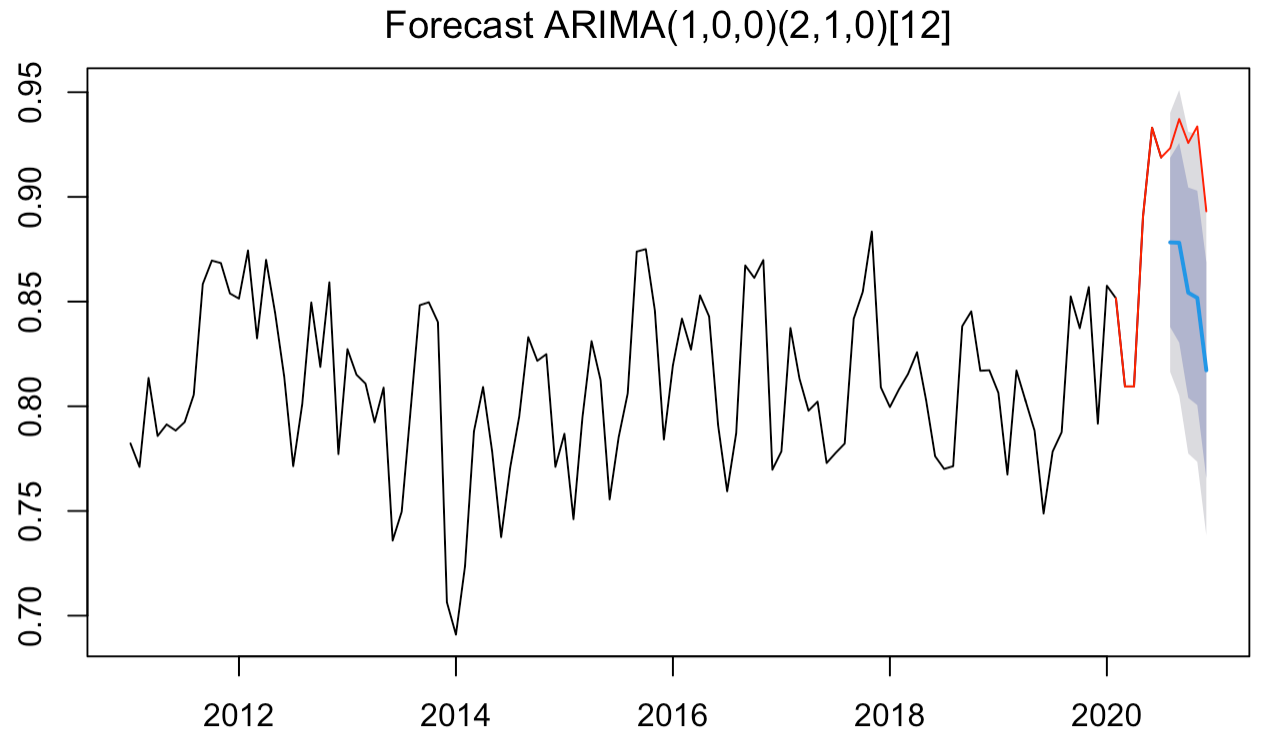
\includegraphics[scale=0.23]{OTRpred.png} \\
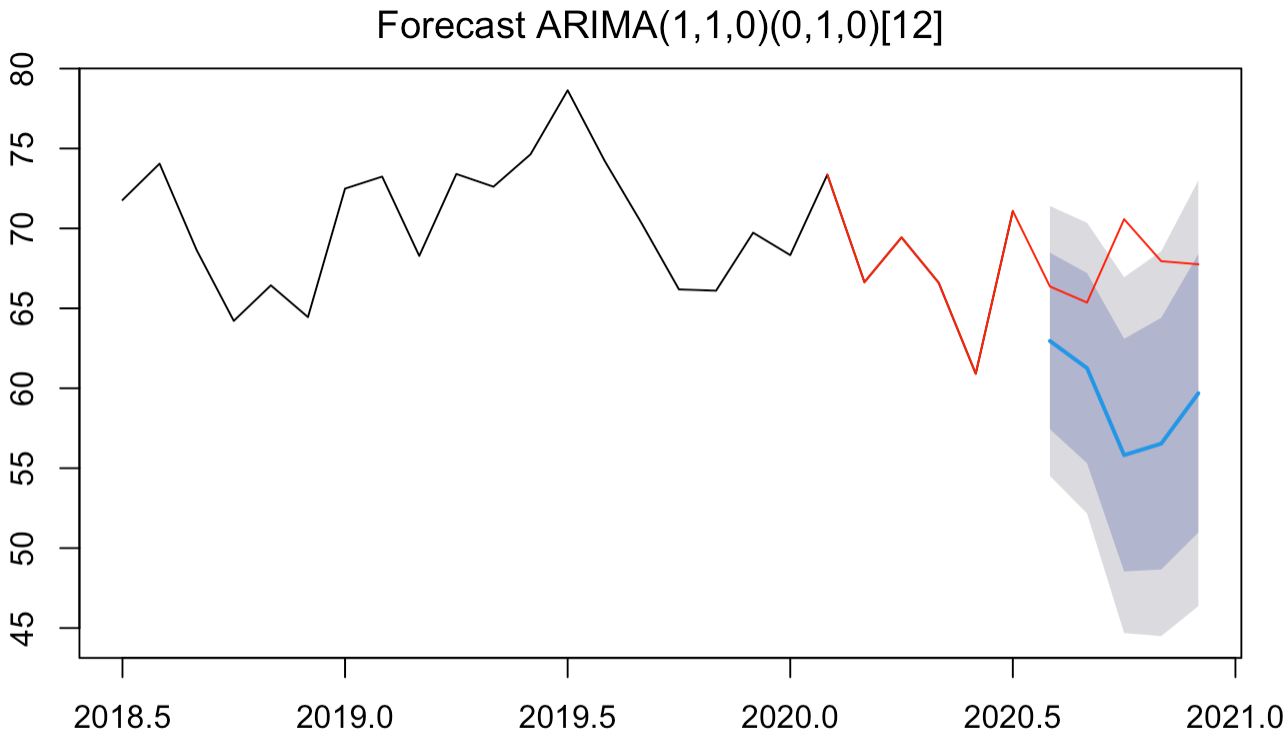
\includegraphics[scale=0.23]{ADMpred.png} 
\caption{Forecasting Plots}
\end{figure}
\end{frame}

\begin{frame} {Future work}
\center
Like Gaussian Mixture Model, can we mix the two models here? \\
\large
Other Questions?
\end{frame}

\begin{frame} {Reference}
\tiny
\begin{itemize}
\item B. Walther, "6 Most Important KPIs For Airline Operations," Information Design, 3 2021. [Online]. Available: https://www.id1.de/2019/10/25/6-most-important-kpis-for-airline-operations-and-performance-analysis/. 
\item "ON-TIME PERFORMANCE OTP IS BECOMING INCREASINGLY IMPORTANT TO AN AIRLINES AND AIRPORTS," OAG Aviation Worldwide Limited, 2021. [Online]. Available: https://www.oag.com/on-time-performance-airlines-airports.\\
\item G. D. Gosling, "Aviation System Performance Measures," UC Berkeley, 1999. [Online]. Available: https://escholarship.org/uc/item/2xw9204x.\\
\item G. a. J. G. Box, Time Series Analysis: Forecasting and Control, San Francisco: Holden-Day, 1970. 
S. Chatterjee, "Time Series Analysis Using ARIMA Model In R," 05 02 2018. [Online]. Available: https://datascienceplus.com/time-series-analysis-using-arima-model-in-r/.
\end{itemize}
\end{frame}

\end{document}